\chapter{Parallel method for generating pairs}
\label{chap:pairs}

A congruence is a binary relation, and therefore is formally described as a set
of pairs.  In a computational setting, it is rarely practical to keep track of
every pair in a congruence; a congruence on a semigroup of size $n$ contains
$n^2$ pairs in the worst case, and on an infinite semigroup contains an infinite
number of pairs.  A congruence can be described in more concise ways:
for example, taking advantage of it being an equivalence relation
and recording only its equivalence classes; or in the case of a Rees congruence,
storing a generating set for the ideal which defines it.  A variety of different
ways to describe a congruence are explained in Chapter \ref{chap:converting},
along with ways to convert from one to another.  However, a congruence is still just
a set of pairs, and by reducing the number of pairs we store, we can often describe a
congruence very concisely using them.

Let $S$ be a semigroup and let $R$ be a subset of $S \times S$.  Recall from
Definition \ref{def:gen-pairs} that the \textit{congruence generated by} $R$ is
the least congruence (with respect to containment) that contains $R$ as a
subset.
This definition is based on a simple intuitive idea:
a congruence $\rho$ is generated by a set of pairs $R$ if it consists
of only the pairs in $R$ along with the pairs required by the axioms of a
congruence (reflexivity, symmetry, transitivity and compatibility).  Thus a
congruence can be described completely by storing only a few pairs.
Indeed, many congruences are \textit{principal}, requiring only one pair to
generate them: see, for example, the congruences studied in Chapter
\ref{chap:motzkin}, most of which are principal.

Another justification for the use of generating pairs is that it is a completely
generic representation.  Some special types of semigroup have their own abstract
representations of congruences -- for inverse semigroups, one can study
kernel--trace pairs \cite[\S 5.3]{howie}; for groups, normal subgroups
\cite[Theorem 11.5]{warner}; for completely simple or completely 0-simple
semigroups, linked triples \cite[\S 3.5]{howie} -- but generating pairs can
represent a congruence on any semigroup whatsoever.  Furthermore, one
might be interested in what pairs are implied by a given pair or set of pairs in
a congruence, and this representation can answer such questions.
Left congruences and right congruences can also be described using generating
pairs, and some algorithms designed for two-sided congruences can be used with
minor modifications to compute information about left and right congruences.

Algorithms for computing a congruence defined by generating pairs have existed
in the \GAP{} library for many years \cite[\texttt{lib/mgmcong.gi}]{gap}, but
lack sophistication and perform slowly (see Section
\ref{sec:random-benchmarking} for benchmarks).  The approach taken in the
library is based on an algorithm in \cite{atkinson_1984} for finding the blocks
of a transitive permutation group: essentially it consists of repeatedly left-
and right-multiplying the generating pairs by generators of the semigroup, and
storing the generated relation in a union--find table (see Section
\ref{sec:union-find}).  This approach is essentially the same as the
\textit{pair orbit enumeration} algorithm that is described in detail in Section
\ref{sec:p}.

This chapter describes a new parallelised approach for computing a congruence
from a set of generating pairs, as implemented in \libsemigroups{}
\cite{libsemigroups}.  First we will give a general outline of the system and
what questions it hopes to answer; then we will describe in detail each
algorithm used, its advantages and disadvantages, and when it can be applied.
Next we will explain how the different algorithms are executed together, and
consider their implementation in \libsemigroups{}; and finally we will show the
results of some benchmarking tests which compare its performance to the code in
the \GAP{} library.

\section{Reasons for parallelisation}

Parallel processing has seen major advances in the last ten years, with
multi-core processors becoming the norm in many types of computers, and
processors with 4, 8, or even 16 cores becoming common on a desktop PC.  This
being the case, it is desirable to parallelise mathematical algorithms wherever
possible, and take advantage of the ability to execute multiple
threads of instructions concurrently.  Some algorithms
are ``embarrassingly parallel'' -- that is, they can be split into
independent threads which require almost no communication with each other.
Examples of these algorithms would be brute force searches, or rendering of
computer graphics.
These are suited so well to parallelisation that splitting the operation into
$n$ parallel threads reduces the expected run-time to barely more than
$\frac{1}{n}$ times the expected run-time in a single thread.  Other
algorithms do not parallelise so well: sometimes threads have to communicate, or
use shared resources, causing significant slowdown and severely limiting the
improvements that can be made by parallelising.

When it comes to computing information about a congruence from generating pairs,
there are various different approaches which can be taken: in Sections
\ref{sec:p}, \ref{sec:tc} and \ref{sec:kb}, we describe three possible
algorithms: pair orbit enumeration, the Todd--Coxeter algorithm, and the Knuth--Bendix algorithm.
Depending on what sort of semigroup is given as an input (see Section
\ref{sec:program-outputs}), several
or all of these might be appropriate.  However, depending on certain properties
of the congruence, one might perform far better than another.  For example, the
pair orbit algorithm works well on congruences that contain few non-reflexive
pairs, while the Todd--Coxeter algorithm tends to work well on congruences with
few classes (i.e.~very many pairs).  For a detailed analysis of which algorithms
perform well on which inputs, see Section \ref{sec:benchmarking}.  Given
only a set of generating pairs, these properties are likely to be unknown in
advance, which makes it difficult to choose a good algorithm.

The natural answer to this problem is the core concept of this chapter: a
parallel approach which does not attempt to parallelise individual algorithms,
but which runs several known algorithms at the same time, each in a different
thread, and simply halts all threads as soon as any one completes.  Since these
algorithms do not interact with each other in any way, the total run-time will
be close to the minimum run-time of all the different algorithms.  This is
particularly important, since for certain semigroups and congruences some
algorithms will never terminate, while others may terminate in a very short
time.

\section{Applicable representations of a semigroup}
\label{sec:applicable-representations-of-a-semigroup}

A semigroup can be represented computationally in different ways.  For example,
a semigroup of transformations could be specified by a set of transformations
that generates it, or alternatively by a finite presentation.
Which representation is used affects which methods will be most effective,
or even which methods will be applicable.  For this purpose, we consider two
different categories of semigroup representation: finitely presentations, and
\textit{concrete} representations.  Recall Section \ref{sec:intro-presentations} for
the definitions of terms surrounding finite presentations.

\begin{definition}
  \label{def:concrete}
  \index{concrete}
  Let $S$ be a semigroup.
  A \textbf{concrete representation} for $S$ is a data structure that can be
  used to:
  \begin{itemize}
  \item produce a list of all the elements of $S$;
  \item produce the product of two elements of $S$;
  \end{itemize}
  in a finite amount of time.
\end{definition}

Note that only finite semigroups can have concrete representations, since we
cannot produce an infinite list of elements in finite time.

There are many different concrete representations for semigroups.  Perhaps the
most trivial and obvious example would be a semigroup's Cayley table (see
Definition \ref{def:cayley-table}).  A Cayley table has a finite number of
rows and columns, and therefore must describe a finite semigroup.  A list of
elements of the semigroup can be taken directly from the indices of the table,
and the product $xy$ of two elements $x$ and $y$ can be found by simply reading
the entry in row $x$ and column $y$.  Hence Cayley tables are concrete, but in
practice in computation they are used very little, since they require a great
deal of space to store -- order $O(|S|^2)$.

It will be more common for us to consider semigroups of partial transformations.
If $S$ is a semigroup of partial transformations, then a set of generators for
$S$ is a concrete representation of $S$.  Two elements can be multiplied and
compared without reference to the semigroup as a whole: for example, if
$x = \transV 13342$ and $y = \transV 24422$ then we can calculate
$xy = \transV 24424$ without knowing anything else about $S$.  So long as all
elements in these semigroups have finite degree, and so long as there are only a
finite number of generators, the semigroup in question will also certainly be
finite, and we can produce a list of its elements using, for example, the
Froidure--Pin algorithm (see Section \ref{sec:find-pres}).  Hence, a
generating set for a semigroups of partial transformations is a concrete
representation.

A finite presentation, on the other hand, is an example of a semigroup
representation that is not concrete.  If $\pres X R$ is a finite presentation,
and $S$ is the semigroup it defines, then it may be that $S$ is infinite, and so
a list of elements of $S$ cannot be produced in finite time -- consider, for
example, the presentation $\pres a \varnothing$ with one generator and no
relations, which presents the free semigroup $\{a\}^+$.  Hence a finite
presentation is not, in general, a concrete representation.

The only guarantee that can be given by the algorithm is that an answer will be
returned if $S$ happens to be finite.  In the concrete case, semigroups are
always finite and so an answer is guaranteed; but in the case of a finitely
presented semigroup, it is unknown in advance whether a semigroup is finite or
not.  Hence, the user of this algorithm might not know whether a particular run
is guaranteed to terminate, since a run that is about to finish is
indistinguishable from one that will run forever.  In some cases, however, we
may be able to return an answer even if $S$ is infinite.  For a fuller
explanation of presentations and decidability issues, see Sections
\ref{sec:intro-presentations} and \ref{sec:computation-decidability}.

Finitely presented monoids are treated as equivalent to finitely presented
semigroups, since a monoid presentation $\pres X R$ can be easily converted into
an equivalent semigroup presentation: an extra generator $\varepsilon$ should be
added to $X$, and relations $(x \varepsilon,x)$ and $(\varepsilon x,x)$ added to
$R$ for each generator $x \in X$.

\section{Program inputs}
\label{sec:program-inputs}

Our algorithm determines the properties of a single left, right, or two-sided
congruence defined by generating pairs, over a semigroup $S$.
For the remainder of this chapter, the word ``congruence'' will be used to refer
to left, right, and two-sided congruences equally, without having the default
meaning of ``two-sided congruence''.

If $S$ has a concrete representation (as described in Section
\ref{sec:applicable-representations-of-a-semigroup}) then we will certainly
have a generating set for $S$; in this case, it is quick to use these generators
to calculate a list of elements in $S$, along with left and right Cayley graphs
for $S$, using the Froidure--Pin algorithm (see Section \ref{sec:find-pres}).
The Froidure--Pin algorithm also gives us, for each element $s \in S$, a word
$w \in X^+$ which \textit{represents} $s$ in the sense of Figure
\ref{fig:word-represents-element}.  We use these words to define a
\textbf{factorisation function} $f : S \to X^+$ which maps each $s$ to its
corresponding word $w$.
\index{factorisation function}

If on the
other hand $S$ is a finitely presented semigroup, then the elements will not be
known in advance.  In either case, a finite presentation $\pres X R$ can be
given -- a technique for efficiently finding a presentation from a concrete
representation is given in Section \ref{sec:find-pres}.
The exact parameters supplied to the algorithm are therefore as follows:
\begin{itemize}
\item A set of generators $X$;
\item A finite set of relations $R \subseteq X^+ \times X^+$;
\item A finite set of generating pairs $W \subseteq X^+ \times X^+$;
\item A record of whether we are computing a left, right, or two-sided
  congruence.
\end{itemize}
The following are also available only in the case of a concrete representation:
\begin{itemize}
\item A list of elements of $S$;
\item Left and right Cayley graphs for $S$ (see Definition
  \ref{def:cayley-graph});
\item A factorisation function $f : S \to X^+$.
\end{itemize}

We shall now make clear the meanings of these different parameters, by giving a
complete description of the system, starting with the commutative diagram in
Figure \ref{fig:pairs-cd-1}.

Here $X$ is our alphabet, and $X^+$ is the free semigroup it defines.  We have a set
of relations $R \subseteq X^+ \times X^+$, which generates the two-sided
congruence $R^\sharp$ on $X^+$.  This two-sided congruence gives rise to a
quotient semigroup $X^+ / R^\sharp$; this is isomorphic to the semigroup $S$,
which is described by the presentation $\pres X R$.  The congruence also gives
us its natural homomorphism $\pi: X^+ \to S$ (see Definition
\ref{def:natural-homomorphism}).  We also have a set of generating pairs
$\mathbf{P} \subseteq S \times S$, which defines a left, right, or two-sided
congruence $\mathbf{P}^\triangleleft$, $\mathbf{P}^\triangleright$, or
$\mathbf{P}^\sharp$.  The aim of the algorithm described in this chapter is to
obtain a data structure describing this congruence, where the precise meaning of
``data structure'' is defined in Section \ref{sec:program-outputs}.  If we are
calculating a two-sided congruence, then it gives rise to the quotient semigroup
$S / \mathbf{P}^\sharp$.

\begin{figure}[ht]
  \centering
  $\begin{tikzcd}
    X \arrow[dr] \arrow[d, hook] & \\
    X^+ \arrow[r, two heads, "\pi"] & \frac{X^+}{R^\sharp} \cong S \arrow[r, two heads] & \frac{S}{\mathbf{P}^\sharp}
  \end{tikzcd}$
  \caption{How input objects relate to each other}
  \label{fig:pairs-cd-1}
\end{figure}

The generating pairs $\mathbf{P}$ are not given by the user.  Since the elements
of $S$ might be unknown (for example if $S$ was specified by a finite
presentation), it would be impractical for the user to specify them precisely.
Instead, the user specifies a set $W$ consisting of pairs of words from
$X^+ \times X^+$, which can be evaluated to pairs of elements in $S \times S$,
giving the set of generating pairs $\mathbf{P}$.
More formally, let
$\Pi: X^+ \times X^+ \to S \times S$ be defined by
$\Pi: (w_1, w_2) \mapsto (w_1\pi, w_2\pi)$, where $\pi$ is the natural
homomorphism from $X^+$ to $S$ mentioned above.  The generating pairs
$\mathbf{P}$ of the congruence are given by $\mathbf{P} = W \Pi$.
This relationship is summarised in Figure \ref{fig:pairs-cd-2}.

\begin{figure}[ht]
  \centering
  $\begin{tikzcd}
    W \arrow[r, two heads, "\Pi|_W"] \arrow[d, hook] & \mathbf{P} \arrow[d, hook] \\
    X^+ \times X^+ \arrow[r, two heads, "\Pi"] & S \times S
  \end{tikzcd}$
  \caption{How generating pairs are specified}
  \label{fig:pairs-cd-2}
\end{figure}

\section{Program outputs}
\label{sec:program-outputs}

Each method we are about to explain can provide a variety of different pieces of
information, but it is important to consider which questions we aim to answer.
Our system should be able to return the following information about a given
congruence when requested:

\begin{enumerate}[(i)]
\item An algorithm to determine whether a given pair $(x,y)$ is in the
  congruence;
\item The number of congruence classes;
\item An algorithm that takes an element $x$ and returns the index of the
  congruence class to which it belongs (it should return the same index for
  elements $x$ and $y$ if and only if $(x,y)$ is in the congruence);
\item A list of the elements in each non-trivial congruence class (only if
  finite).
\end{enumerate}

Each of our algorithms will produce a data structure which allows us to answer
each of these questions.  After each algorithm is described in Section
\ref{sec:methods}, we will explain how that algorithm can be used to produce
each of these four pieces of information.  Note however that item (iv) can only
be produced by an algorithm if the list happens to be finite -- that is, only if
all but finitely many elements of the semigroup lie in singletons.

\section{Finding a presentation}
\label{sec:find-pres}

Recall from Section \ref{sec:program-inputs} that a concrete representation for
a semigroup may not include a finite presentation.  In order to use the Todd--Coxeter and
Knuth--Bendix algorithms, a finite presentation is required, and so a presentation
$\pres X R$ must be calculated for $S$.  For the purposes of the algorithm
described in this chapter, it is not important how this presentation is
obtained.  However, for the sake of completeness, we will briefly discuss how a
presentation could be computed.

We will start by describing a very simple way of producing a presentation from a
concrete representation: by using its Cayley table directly.

\begin{method}
  \label{meth:trivial-presentation}
  Let $S$ be a semigroup with concrete representation, and assume we have access to its Cayley
  table.  We can produce a presentation as follows.  Let $\bar S$ be a set with
  the same cardinality as $S$, containing an element $\bar{x}$ for each element
  $x \in S$, and let $R \subseteq \bar{S} \times \bar{S}$ be defined by
  $\{(\bar{x}\bar{y}, \overline{xy}) : (x,y) \in S \times S\}.$ The resulting
  presentation $\pres{\bar{S}}{R}$ defines the semigroup $S$.

  \begin{proof}
    Consider the natural homomorphism $\pi: \bar{S}^+ \to S$ which maps a word
    $\bar{x}_1\bar{x}_2\ldots \bar{x}_n$ to the semigroup element
    $x_1 x_2\ldots x_n$.
    Note that $\pi$ is surjective, since for any element $x \in S$ we have
    $(\bar{x})\pi = x$.
    To prove that $\pres{\bar{S}}{R}$ defines $S$ we must
    show that for any two words $u, v \in \bar{S}^+$, $(u, v) \in R^\sharp$ if
    and only if $(u)\pi = (v)\pi$.

    Let $u,v \in \bar{S}^+$ such that $(u, v) \in R^\sharp$.  As in Theorem
    \ref{thm:rsharp}, there must be a chain of words
    $$u = w_1 \to w_2 \to \cdots \to w_k = v$$
    such that $w_i = xay$ and $w_{i+1} = xby$ for some words $x,y \in \bar{S}^*$ and
    $a,b \in \bar{S}^+$ where either $(a,b)$ or $(b,a)$ is in $R$, for each
    $i \in \{1, \ldots, k-1\}$.  In each of these steps, $(a,b)$ or $(b,a)$
    being in $R$ implies that $(a)\pi = (b)\pi$, because of the way in which $R$
    was created.  Since $\pi$ is a homomorphism, this tells us that
    $(xay)\pi = (xby)\pi$, and therefore that $(u)\pi = (v)\pi$, proving this
    implication.

    For the converse, let $u,v \in \bar{S}^+$ such that $(u)\pi = (v)\pi$.  Let
    $u = \bar{u}_1\bar{u}_2\ldots \bar{u}_k$ and $v = \bar{v}_1\bar{v}_2\ldots \bar{v}_l$, with each $\bar{u}_i$ and $\bar{v}_j$
    being from $\bar{S}$.  Since $R$ has a relation $(\bar{x}\bar{y}, \overline{xy})$ for each
    pair $(\bar{x},\bar{y}) \in \bar{S} \times \bar{S}$, there exists a relation
    $(\bar{u}_1\bar{u}_2, \overline{u_1u_2}) \in R$, and so by repetition we have
    $(u, u') = (\bar{u}_1\bar{u}_2\ldots \bar{u}_k, \overline{u_1u_2\ldots u_k}) \in R^\sharp$, relating the
    word $u$ with length $k$ to a word $u'$ with length $1$, such that
    $(u)\pi = (u')\pi$.  We can perform
    a similar process on $v$ to produce a word $v'$ also with length $1$, with
    $(v)\pi = (v')\pi$.
    Since $(u')\pi = (u)\pi = (v)\pi = (v')\pi$ and both $u'$ and $v'$
    have length $1$, we must conclude that $u' = v'$, and so we
    find that
    $$u ~R^\sharp~ u' = v' ~R^\sharp~ v,$$
    so $(u,v) \in R^\sharp$ as required.
  \end{proof}
\end{method}

Consider the following example.

\begin{example}
  Let $\T_2$ be the full transformation semigroup on $2$ points.  It has $4$
  elements,
  $$\left\{\transII 12, \transII 21, \transII 11, \transII 22\right\},$$
  which we will relabel as $\{a,b,c,d\}$.  The Cayley table is
  $$
  \begin{array}{c | c c c c}
    & a & b & c & d \\
    \hline
    a & a & b & c & d \\
    b & b & a & c & d \\
    c & c & d & c & d \\
    d & d & c & c & d \\
  \end{array}
  $$
  The method from Proposition \ref{meth:trivial-presentation} converts this
  Cayley table to the presentation
  \begin{alignat*}{7}
    \langle\, a,b,c,d ~|~
    aa&=a,\ & ab&=b,\ & ac&=c,\ & ad&=d, \\
    ba&=b,\ & bb&=a,\ & bc&=c,\ & bd&=d, \\
    ca&=c,\ & cb&=d,\ & cc&=c,\ & cd&=d, \\
    da&=d,\ & db&=c,\ & dc&=c,\ & dd&=d\,\rangle,
  \end{alignat*}
  which has $4$ generators and $16$ relations.
\end{example}

This approach is simple to describe, but of course results in a large, unwieldy
presentation which will be difficult to use in computations: it will have $|S|$
generators and $|S|^2$ relations, which is likely to be far more than necessary,
and will therefore slow down the Todd--Coxeter and Knuth--Bendix algorithms badly.
If $S$ is $\T_5$, the full transformation semigroup on $5$ points, it has only
$3125$ elements, but the presentation produced would have $3125$ generators and
$9,765,625$ relations, an absurdly large representation for a semigroup which
can be generated by just three transformations of degree $5$.  We
therefore might consider an alternative.

% $\T_5 = \langle \transV23451, \transV21345, \transV12341 \rangle$

If $S$ has a known generating set $X$, we can use it to produce a presentation
which is likely to much smaller.  Consider the following approach, which is
adapted from the simplified version of the algorithm shown in
\cite[\S 3.1]{froidure_pin}, where its correctness is proven in more detail.

\begin{method}
  \label{meth:inbetween-presentation}
  Let $S$ be a finite semigroup with a concrete representation, and let
  $X \subseteq S$ be a generating set for $S$.  We can produce a presentation
  $\pres X R$ consisting of the known generating set $X$ together with some
  relations $R$ which are computed as follows, with complete pseudo-code in
  Algorithm \ref{alg:inbetween-presentation}.

  Let $R$ begin empty (line 2), and start enumerating the elements of the monoid $S^1$.
  We keep a list $L_S$ of elements that have been found in $S^1$ (initially just
  the identity $\id$, as in line 3), and we keep another
  list $L_{X^*}$ of words made up of generators from $X$ (initially just the
  empty word $\varepsilon$, as in line 4).  We also define a
  function $\nu : X^* \to S^1$ which maps a word $w=x_1x_2\ldots x_n$ to the
  element $x_1\cdot x_2\cdots x_n$ found by multiplying the generators (and
  $\varepsilon \mapsto \id$ as a special case).
  We now loop over the words $w$ that have been found and added to $L_{X^*}$;
  initially this list contains only one word, but in each iteration of the loop,
  we may discover new words, which we add to the end of the list, and iterate
  over in course, until we have considered all words (line 16).

  In each iteration of the loop, we take the next word $w \in L_{X^*}$ (line 8)
  and for each generator $x \in X$ in turn we consider the new word $wx$ made by
  appending $x$ to the end of $w$.  If this new word represents an element of
  $S^1$ that has already been found -- that is, if $(wx)\nu \in L_S$ -- then we
  add a new relation $(wx, w')$ to $R$, where $w'$ is the word we have already
  stored that represents $(wx)\nu$ (line 12).  If, on the other hand, this new
  word does not represent an element that we already know, then we have
  encountered a new element which must be added to $L_S$ (line 14) and we have a
  word that represents it, which must be added to $L_X*$ (line 15).

  Once the loop is run to the end, this if--else statement (lines 10--15)
  ensures that every word $w \in X^*$ can be rewritten by a relation in $R$ to a
  word in $L_{X^*}$, and that every element in $S$ has precisely one word in
  $L_{X^*}$ which represents it.
  Hence the resulting presentation $\pres X R$ defines the semigroup $S$.

  We can also see that this algorithm always terminates for finite $X$ and
  finite $S$: the repeat-loop is only run once for each element of $S$, and the
  for-loop inside is only run once for each generator in $X$.  Hence the loop
  must complete, and the algorithm halts.
\end{method}

\begin{algorithm}
\caption{The \textsc{PresentationFromGenerators} algorithm}
\label{alg:inbetween-presentation}
\index{PresentationFromGenerators@\textsc{PresentationFromGenerators}}
  \begin{algorithmic}[1]
    \Procedure{PresentationFromGenerators}{$X$}
      \State $R := \varnothing$
      \State $L_S := \{\id\}$
      \State $L_{X^*} := \{\varepsilon\}$
      \State $i := 0$  \Comment{Number of words we have looped over}
      \Repeat
      \State $i \gets i + 1$
      \State $w :=$ the $i$th element of $L_{X^*}$
        \For{$x \in X$}
          \If{$(wx)\nu \in L_S$}  \Comment{New word for known element}
          \State $w' :=$ the unique element in $L_{X^*}$ such that $(w')\nu = (wx)\nu$
            \State Add $(wx, w')$ to $R$
          \Else  \Comment{Previously unknown element}
            \State Add $(wx)\nu$ to $L_S$
            \State Add $wx$ to $L_{X^*}$
          \EndIf
        \EndFor
      \Until{$i = |L_{X^*}|$}  \Comment{There are no words left to consider}
      \State \Return $\pres X R$
    \EndProcedure
  \end{algorithmic}
\end{algorithm}

We can improve further on this method.  The \libsemigroups{}
implementation of this chapter's algorithm uses the Froidure--Pin algorithm
\index{Froidure--Pin}
\cite{froidure_pin}, a method which is essentially a more advanced variation of
Algorithm \ref{alg:inbetween-presentation}.  The Froidure--Pin algorithm takes a concrete set of
generators $X$ for a semigroup $S$, and returns several useful pieces
of information:
\begin{itemize}
\item a left Cayley graph for $S$ with respect to $X$;
\item a right Cayley graph for $S$ with respect to $X$;
\item a confluent terminating rewriting system $R$ describing the elements of
  $S$ as words in $X^+$;
\item and for each element $s \in S$, a word $w \in X^+$ representing one
  possible factorisation of $s$.
\end{itemize}
The right Cayley graph can be used by the Todd--Coxeter procedure to pre-fill its
table (see Section \ref{sec:tc-prefill}).  But more importantly, the rewriting
system $R$ is a set of pairs which can be used as the relations in a finite
presentation $\pres X R$ for the semigroup $S$.
Rewriting systems will be defined later in Section \ref{sec:kb}, along with the
terms ``confluent'' and ``terminating''.  The fact that $R$ is confluent
and terminating may also be useful when it is used as part of a rewriting system
in the Knuth--Bendix process, as we will see in Theorem \ref{thm:kb-halt}.

A full description of the Froidure--Pin algorithm is outside the scope of this
thesis, but for more information about the algorithm and its implementation in
\libsemigroups{}, see \cite{froidure_pin} and \cite{froidure_pin_jonusas}.

The presentation produced by the algorithms above presents a finite semigroup,
and therefore has decidable word problem.  Hence, when we have a concrete
representation for a semigroup $S$, we can always find a presentation in which
we can compare two words and say whether they represent the same element of $S$.
However, if we started with a finite presentation instead of a concrete
representation, we may not have this guarantee.  There are many examples of
presentations for which the word problem is undecidable (see Examples
\ref{ex:makanin} and \ref{ex:cijtin}). Many presentations do have decidable word
problem (see Example \ref{ex:presentation-decidable}), but many do not, and
there is no algorithm to decide whether a given presentation does.  Besides,
finite presentations, even if their word problem is decidable, can describe
infinite semigroups, and the finiteness of $S$ is also not known in advance --
nor, in general, is it decidable.

\section{The methods}
\label{sec:methods}

\subsection{Pair orbit enumeration}
\label{sec:p}
\index{pair orbit enumeration}

The first method we will describe is \textit{pair orbit enumeration}.  This
rather simple algorithm consists of taking the pairs in $\R$, and for each pair
$(a,b)$ finding all pairs $(as, bs)$ and $(sa, sb)$ for all $s \in S$.  We might
refer to this set of pairs as the \textit{orbit} of $\R$ in $S$, which justifies
the name.  Although this algorithm is simple and in some ways inefficient, there
are cases in which it out-performs the other algorithms in this chapter, so it
is worth including in our parallelised method.

We will now give a brief description of pair orbit enumeration -- a pseudo-code
description is shown in Algorithm \ref{alg:p}.  We start with a semigroup $S$, a
set of generators $X$ for $S$, and a set of generating pairs $\mathbf{R}$ for
the congruence $\rho$ we are trying to compute.  It will also be important to
remember whether we are calculating a left, right, or two-sided congruence, a
piece of information encoded in Algorithm \ref{alg:p} as $\sigma \in \{L,R,T\}$.
We start with a list of pairs $\mathbf{R}'$ which we initialise to be equal to
the set of generating pairs $\mathbf{R}$ (line 3); this list $\mathbf{R}'$ will hold all
the pairs that have been found so far, except those we infer from reflexivity,
symmetry and transitivity.  We will also create a union--find table
$(\Lambda,\tau)$ for storing the classes (line 4), and we will be using the three
operations \textsc{AddElement}, \textsc{Union} and \textsc{Find} to modify them.
See Section \ref{sec:union-find} for a full description of the union--find
method.

Now we can describe the overall structure of the pair orbit enumeration method.
We begin iterating through the pairs in $\mathbf{R}'$ (the repeat loop starting on line 6), and as we do so we
will add further pairs to $\mathbf{R}'$ which will also need to be iterated on,
until we reach the end of the list (line 19).  For each pair $(a,b)$ we first need to
merge the congruence classes of $a$ and $b$ in the union--find table using
\textsc{Union} (line 13).  However, if either $a$ or $b$ is not
already in $\Lambda$, then it will need to be added first using \textsc{AddElement} (lines 9--12).  Now,
for each generator $x$, we can find the two pairs $(xa,xb)$ and $(ax,bx)$.
Depending on whether we are calculating a left, right, or two-sided congruence
(that is, depending on the value of $\sigma$)
we add one or both of these pairs to $\mathbf{R}'$ to be processed in its own
turn (lines 16 and 18).

\begin{algorithm}
\caption{The \textsc{PairOrbit} algorithm}
\label{alg:p}
\index{PairOrbit@\textsc{PairOrbit}}
\begin{algorithmic}[1]
\Require $S$ a semigroup,
         $\mathbf{R} \subseteq S \times S$,
         $\sigma \in \{L, R, T\}$
\Procedure{PairOrbit}{$S, \mathbf{R}, \sigma$}
\State Let $X$ be a generating set for $S$
\State $\mathbf{R}' := \mathbf{R}$
%\Comment{$\mathbf{R}'$ is the list of pairs found so far}
\State $(\Lambda, \tau) := (\varnothing, \varnothing)$
\Comment{An initialised union--find table}
\State $i := 0$  \Comment{Number of pairs we have looped over}
\Repeat
  \State $i \gets i + 1$
  \State $(a,b) :=$ the $i$th pair in $\mathbf{R}'$
  \If{$a \notin \Lambda$}
    \State \Call{AddElement}{$a$}
  \EndIf
  \If{$b \notin \Lambda$}
    \State \Call{AddElement}{$b$}
  \EndIf
  \State \Call{Union}{$a, b$}
  \For{$x \in X$}
    \If{$\sigma \in \{L, T\}$}
      \State Add $(xa, xb)$ to $\mathbf{R}'$ if not already present
    \EndIf
    \If{$\sigma \in \{R, T\}$}
      \State Add $(ax, bx)$ to $\mathbf{R}'$ if not already present
    \EndIf
  \EndFor
\Until{$i = |\mathbf{R}'|$}  \Comment{There are no pairs left to process}
\State \Return $(\Lambda, \tau)$
\EndProcedure
\end{algorithmic}
\end{algorithm}

Once this procedure is finished, we have a complete table $(\Lambda,\tau)$ which describes
the congruence's non-trivial classes.  To check whether a pair $(a,b)$ lies in
the congruence, we now just need to look up $a$ and $b$ in the table using
\textsc{Find}, and if they lie in the same class we return true.  If either
element has not been added to $\Lambda$, then it lies in a singleton, and $(a,b)$
is in the congruence if and only if $a=b$.

In order to prove that this method is valid, we will recall some facts from
Chapter \ref{chap:intro}, as well as citing several sources for some theory.
Let $S$ be a semigroup, let $\mathbf{R} \subseteq S \times S$, let
$\sigma \in \{L, R, T\}$, and let $\rho$ be the left, right or two-sided
(according to $\sigma$) congruence on $S$ generated by $\mathbf{R}$.  We can now
state the following theorem.

\begin{theorem}
  \label{thm:p}
  Let $(\Lambda, \tau) = \textsc{PairOrbit}(S, \mathbf{R}, \sigma)$.  Distinct elements
  $x$ and $y$ in $\Lambda$ lie in the same class of $\rho$ if and only if
  $\textsc{Find}(x) = \textsc{Find}(y)$.
  \begin{proof}
    Recall from Definition \ref{def:rc} the relations $\mathbf{R}^c$,
    $\mathbf{R}^l$ and $\mathbf{R}^r$, and recall that they are respectively the
    smallest compatible, left-compatible, and right-compatible relations which
    contain $\mathbf{R}$ (see Lemma \ref{lem:rc}).

    Let us start by considering the case when $\sigma = L$, that is the case
    where we are computing the left congruence.  For each pair
    $(a,b) \in \mathbf{R}$, the pair orbit enumeration procedure finds all the
    pairs $(xa, xb)$ where $x$ is a generator of $S$.  That pair is then added
    to $\mathbf{R}'$ (line 16), and so it is kept in line for processing.  On a
    later run through the repeat loop, when $i$ is incremented in line 7 and
    reaches the position of $(xa, xb)$ in $\mathbf{R}'$, $(xa, xb)$ is
    considered as a pair in its own right, and all of its left multiples are
    found in their turn: $(yxa, yxb)$ for every generator $y \in X$.  In this
    way, $(sa, sb)$ is found for every
    $s \in S$, so the set of pairs found by the \textsc{PairOrbit} algorithm is
    $$\{(sa, sb) ~|~ (a,b) \in \mathbf{R}, s \in S\},$$
    which is equal to the relation $\mathbf{R}^l$.
    Similarly, if $\sigma = R$, the algorithm finds all the pairs in
    $\mathbf{R}^r$, and if $\sigma = T$, the algorithm finds all the pairs in
    $\mathbf{R}^c$.

    The remainder of the proof considers the union--find method.  As described
    above, since union--find stores pairs as a partition, it automatically takes
    care of reflexivity, symmetry, and transitivity.  That is, if a set of pairs
    $Q$ is fed into the union--find table using \textsc{Union} on every pair in
    $Q$, then the resulting table describes $Q^e$, the least equivalence
    relation containing $Q$.  Hence, if $\sigma = L$, the table produced by
    $\textsc{PairOrbit}$ will describe the relation $(R^l)^e$; if $\sigma = R$, it will
    describe $(R^r)^e$; and if $\sigma = T$, it will describe $(R^c)^e$.  As we
    know from Theorem \ref{thm:rsharp}, these relations are respectively the least
    left, right, and two-sided congruence containing $\mathbf{R}$, so the output
    of \textsc{PairOrbit} describes $\rho$ accurately, and \textsc{Find} may be used as
    described to determine whether two elements lie in the same congruence class.
  \end{proof}
\end{theorem}

In \textsc{PairOrbit}, we call \textsc{AddElement}, and thus add
elements to $\Lambda$, only when an element is found in a pair.
This approach opens up the possibility of applying this method to infinite
semigroups.  Our implementation in \libsemigroups{} \cite{libsemigroups}
includes such a possibility, by taking a semigroup presentation $\pres X R$ and
using the Knuth--Bendix algorithm (see Section \ref{sec:kb}) as a way of comparing the semigroup's
elements.  The pair orbit enumeration procedure, as described above, can then be
used, and will complete in finite time if and only if the number of elements in
non-trivial congruence classes is finite.  It should be noted that we can rely
on \textsc{PairOrbit} terminating in a finite number of steps so long as $S$ and
$X$ are finite.  There are only two loops in the algorithm: the inner for-loop
is limited by the finite length of $X$, so it has only a finite number of steps;
and the outer repeat loop can only be run at most $|S|^2$ times, since it runs
once for each pair added to $\mathbf{R}'$, which is a subset of $S \times S$ --
note that new pairs are only added if they are not already present (lines 16 and
18).

This is the simplest of the algorithms discussed in this section, and generally
does not perform as well as the others in practice.  However, it has certain
advantages such as its small overhead and quick setup, and therefore on certain
examples performs better than the others.  Furthermore, it is applicable to any
problem discussed in this chapter, whether we have a concrete representation or
a finite presentation, and whether $\rho$ is a left, right or two-sided
congruence.  Uniquely among the methods described in this chapter, it does not
even require a presentation in order to be run.

Now that we have explained the pair orbit algorithm, we should consider how it
can be used to answer the questions in Section \ref{sec:program-outputs}.
Assume we have a congruence $\rho$ on a semigroup $S$, and the pair orbit
algorithm has been completed.  For (i), we can determine whether a given pair $(x,y)$
lies in $\rho$ fairly easily using the resultant union--find table: $(x,y) \in
\rho$ if and only if $\textsc{Find}(x) = \textsc{Find}(y)$.  For (ii), to find the number
of congruence classes of $\rho$, we first find the number of different blocks in
the union--find table (that is, the number of different values returned by
\textsc{Find} when given elements in $\Lambda$), and then we add the number of
singletons (that is, the number of elements not in $\Lambda$).  Hence the number
of congruence classes of $\rho$ is equal to
$$|\{\textsc{Find}(x): x \in \Lambda\}| + |S \setminus \Lambda|.$$
For (iii), we require an algorithm that takes an element and returns a unique
integer corresponding to the congruence class in which it lies; we can simply
use the function $\textsc{Find}$ and create a map of outputs to integers over
successive calls.  Finally for (iv) we require a list of the
elements in each non-trivial congruence class; this can be produced by calling
\textsc{Find} on each element $x$ in $\Lambda$, and putting $x$ into a list
labelled $L_i$ where $i = \textsc{Find}(i)$, creating new lists as necessary --
once all elements have been considered, these lists are what is required.

This algorithm has rather high complexity.  As we saw in the proof of Theorem
\ref{thm:p}, the algorithm adds pairs to $\R'$ until it is equal to $\R^c$ (for
a two-sided congruence -- substitute $\R^l$ or $\R^r$ for a left or right
congruence).  The repeat-loop will be therefore be executed once for each pair
in $\R^c$, and it contains a for-loop that iterates over $X$.  Hence, even if we
treat calls to \textsc{Union} as close to constant time (see Theorem
\ref{thm:ackermann}) we can only say that \textsc{PairOrbit} has time complexity
order $O(|\R^c| \cdot |X|)$.  Hence, the algorithm can complete quite quickly
for congruences which have a small generating set $X$ and only a few pairs in
$\R^c$ (that is, with many classes).  However, in the worst case, when the
generating set is large and there are many pairs in $\R^c$, the time complexity
is order $O(|S|^3)$, since $\R^c = S \times S$ and $X = S$.  Similarly, to store
all the pairs that are found in $\R^c$ the space complexity in this worst case
is $O(|S|^2)$.  This makes the algorithm unattractive for congruences with many
pairs, but in some cases the algorithm can still out-perform the others in this
chapter (see Section \ref{sec:benchmarking}).

Some improvements can be made to the basic algorithm shown above.  For example,
the \libsemigroups{} implementation makes use of the symmetry of pairs: a
pair $(a,b)$ is not added to $\mathbf{R}'$ if the pair $(b,a)$ has previously
been added.  Tweaks like this can make the algorithm slightly faster, though
they do not address the high complexity of the method.

\subsection{The Todd--Coxeter algorithm}
\label{sec:tc}
\index{Todd--Coxeter}

The Todd--Coxeter algorithm was originally described in 1936 in
\cite{todd_coxeter_1936}.  It was an algorithm to enumerate the cosets of a
finitely generated subgroup of a finitely presented group.  Arriving before the
advent of electronic computers, the algorithm was originally intended to be
carried out by hand.  Perhaps the earliest automatic implementation was on the
EDSAC II computer in Cambridge \cite{leech_1963}.  Since then, a wide variety of
efficient, optimised versions have been implemented, one notable example being
\ACE{} \cite{ace}.

A variation of the Todd--Coxeter algorithm for semigroups was described in 1967
\cite{neumann_1967}.  The algorithm takes a presentation $\pres X R$
for a semigroup $S$ and computes the right regular representation of $S^1$ with
respect to the generators $X$ -- that is, it computes all the elements of $S$ and
the result of right-multiplying each element by each generator (see Section
\ref{sec:transformations}).  Since the
original algorithm makes very little use of those properties unique to groups,
the method applied to semigroups is essentially the same.  Other descriptions of
the Todd--Coxeter algorithm for semigroups can be found in \cite[Chapter 12]{ruskuc_thesis} and
\cite[Chapter 1.2]{walker_thesis}, and a variation specific to inverse
semigroups can be found in \cite{cutting_thesis}.  Our version of the algorithm
is based closely on an implementation by G\"otz Pfeiffer, found in
\cite[\texttt{lib/tcsemi.gi}]{gap}, itself based on \cite{walker_thesis}.

We will now describe the Todd--Coxeter method as used in the context of this
chapter.  Though the Todd--Coxeter method itself does not represent new work, it is an
important part of the overall parallel approach, and in order to understand its
uses and limitations, it is described here in full.
The idea of pre-filling the table is original work (see ``Pre-filling the
table'' below), as is the integration into the overall parallel algorithm this
chapter describes.

\subsubsection{Setup}

The Todd--Coxeter algorithm is based on a table, where each row corresponds to a
single congruence class (or equivalently in the case of a two-sided congruence,
a single element of the quotient
semigroup).  The columns of the table correspond to the generators of the
semigroup, and the entry in row $i$, column $j$ represents the element found by
taking element $i$ and right-multiplying it by generator $j$.  These entries may
be blank, and two different rows may be found to describe the same element.
Mathematically, we can view this table as a triple $(n, \mathbf{N}, \tau)$
consisting of:
\begin{itemize}
\item an integer $n \in \mathbb{N}$ representing the number of rows in the table;
\item a set $\mathbf{N} \subseteq \{1, \ldots, n\}$ containing the indices of the
  \textit{undeleted} rows; and
\item a function $\tau: \mathbf{N} \times X \to \mathbf{N} \cup \{0\}$, where
  $(i, x)\tau$ is equal to the entry in row $i$ and the column corresponding to
  generator $x$ -- with $0$ representing a blank entry.
\end{itemize}

Suppose that we have a semigroup presentation $\pres X R$ for a semigroup
$S$.  The table is initialised with a single row, numbered $1$.  This row
corresponds to the empty word $\varepsilon$, or the adjoined identity of the
monoid $S^1$.  The row is empty, containing a blank entry in all $|X|$ columns.
In our mathematical notation, we define $n=1$ and
$(1,x)\tau = 0$ for all $x \in X$.

We can naturally extend the function
$\tau: \mathbf{N} \times X \to \mathbf{N} \cup \{0\}$
to a function
$\bar{\tau}: \mathbf{N} \times X^* \to \mathbf{N} \cup \{0\}$
which is described as follows.
If $w \in X^*$ and $w=w_1 \ldots w_n$, where $w_1, \ldots, w_n \in X$,
then we can define $\bar\tau$ recursively by
$$
(i, w)\bar\tau = \left\{
\begin{matrix*}[l]
  i & \textnormal{if~} w=\varepsilon,\\
  0 & \textnormal{if~} (i, w_1)\tau=0,\\
  \big((i, w_1)\tau, w_2 \ldots w_n\big)\bar\tau & \textnormal{otherwise}.
\end{matrix*} \right.
$$
The effect of $\bar\tau$ is to trace an entire word through the table, starting
at a given row.

\subsubsection{Elementary operations}

We now describe 3 operations which may be applied to the table.  These
operations will be described in turn to give an understanding of what they are
designed to do, along with their description in pseudo-code
(Algorithms \ref{alg:add}, \ref{alg:trace} and \ref{alg:coinc}).  We will then
describe the overall Todd--Coxeter procedure which uses these operations
to find all the elements of a semigroup from a presentation
(Algorithm \ref{alg:tc}).

\begin{itemize}
\item \textsc{Add}: Fill in a blank entry and add a row to the table;
\item \textsc{Trace}: Trace a relation from a row;
\item \textsc{Coinc}: Process a coincidence.
\end{itemize}

The first operation, \textsc{Add}, is the simplest of the three, and is shown in
pseudo-code in Algorithm \ref{alg:add}.  Calling $\textsc{Add}(i,x)$ should fill
in a blank cell in the table in row $i$ and column $x$ -- that is, a position
such that $(i,x)\tau = 0$.  It fills it in with the address of a new row, which
must first be created.  We add a new row at the bottom of the table by
incrementing the number of rows $n$ (line 2), adding its new value to the list
of active rows $\mathbf{N}$ (line 3), and filling in all its entries with blanks
-- that is, setting its $\tau$-outputs to 0 (lines 4--5).  Finally, the address
of the new row is written into the blank cell that was specified -- that is, we
set $(i,x)\tau$ to the new row's address $n$ (line 6).  Now the blank cell has
been filled with the address of a new row, as required.

\begin{algorithm}
\caption{The \textsc{Add} algorithm (Todd--Coxeter)}
\label{alg:add}
\index{Add@\textsc{Add}}
\begin{algorithmic}[1]
\Require{$(i,x)\tau = 0$}
\Procedure{Add}{$i, x$}
\State $n \gets n + 1$
\State $\mathbf{N} \gets \mathbf{N} \cup \{n\}$
\For{$x \in X$}
  \State $(n, x)\tau := 0$
\EndFor
\State $(i, x)\tau \gets n$
\EndProcedure
\end{algorithmic}
\end{algorithm}

\textsc{Trace} takes two arguments: a row $e$ in the table, and a relation $v=w$
from $R$.  Its goal is to ensure that, starting at $e$, applying the word $v$
has the same result as applying the word $w$ -- in other words, to ensure that
$(e,v)\bar\tau = (e,w)\bar\tau$.  We will now describe how this is done, referring to
Algorithm \ref{alg:trace} for pseudo-code.

First we follow both words through the table, one letter at a time, up to and
including their penultimate letter.  For $v$, we use a variable $s$, which
starts at $e$ (line 4) and we go through $v$ one letter $v_i$ at a time up to
the second-last letter (line 5).  At each step, we consider $(s, v_i)\tau$, the
entry in the table which we must follow next to continue going through the
word.  If it is not set, we call \textsc{Add} to create a new row to point it
towards (lines 6--7).  Then we follow it, setting $s$ to the new value (line
8).  At the end of this loop, we only need to follow the last letter $v_m$ to
complete the word -- that is, $(s, v_m)\tau = (e, v)\bar\tau$.

We follow a similar process for $w$ in lines 9--13, going through all letters of
$w$ except the last one, and finding a row $t$ such that
$(t, w_n)\tau = (e, w)\bar\tau$.  Now in order to satisfy the objective
$(e,v)\bar\tau = (e,w)\bar\tau$, we just need to ensure that two specific cells
in the table are equal: we need to ensure that $(s, v_m)\tau = (t, w_n)\tau$.
We do this by considering four different cases:
\begin{itemize}
\item if the two cells are both empty, then we apply \textsc{Add} to
  $(s, v_m)\tau$ to create a new row for it to point to, and then we copy that
  entry into $(t, w_n)\tau$ (lines 14--16);
\item if just one of the entries is empty, then the filled entry is copied into
  the empty one (lines 17--20);
\item if both entries are filled and equal, we do not need to do anything;
\item if both entries are filled and are distinct, then we need to force the two
  rows they point towards to be equal, by applying \textsc{Coinc} to the two
  entries (lines 21--22).
\end{itemize}
After each of these cases, the result is that $(s, v_m)\tau = (t, w_n)\tau$, and
hence that $(e, v)\bar\tau = (e, w)\bar\tau$ as required.

\begin{algorithm}
\caption{The \textsc{Trace} algorithm (Todd--Coxeter)}
\label{alg:trace}
\index{Trace@\textsc{Trace}}
\begin{algorithmic}[1]
\Procedure{Trace}{$e, v = w$}
\State Write $v = v_1 \ldots v_m$ \Comment $(v_i \in X \text{~for~} 1 \leq i \leq m)$
\State Write $w = w_1 \ldots w_n$ \Comment $(w_i \in X \text{~for~} 1 \leq i \leq n)$
\State $s \gets e$
\For{$i \in \{1, \ldots, m-1\}$}
  \If{$(s, v_i)\tau = 0$}
    \State \Call{Add}{$s, v_i$}
  \EndIf
  \State $s \gets (s, v_i)\tau$
\EndFor
\State $t \gets e$
\For{$i \in \{1, \ldots, n-1\}$}
  \If{$(t, w_i)\tau = 0$}
    \State \Call{Add}{$t, w_i$}
  \EndIf
  \State $t \gets (t, w_i)\tau$
\EndFor

\If{$(s, v_m)\tau = (t, w_n)\tau = 0$}
  \State \Call{Add}{$s, v_m$}
  \State $(t, w_n)\tau \gets (s, v_m)\tau$
\ElsIf{$(s, v_m)\tau = 0$}
  \State $(s, v_m)\tau \gets (t, w_n)\tau$
\ElsIf{$(t, w_n)\tau = 0$}
  \State $(t, w_n)\tau \gets (s, v_m)\tau$
\ElsIf{$(s, v_m)\tau \neq (t, w_n)\tau$}
  \State \Call{Coinc}{$(s, v_m)\tau, (t, w_n)\tau$}
\EndIf

\EndProcedure
\end{algorithmic}
\end{algorithm}

\textsc{Coinc} is used when two rows in the table are found to refer to the same
element of $S$; it modifies the table to delete one row and use the other
instead.  Pseudo-code for \textsc{Coinc} can be found in Algorithm
\ref{alg:coinc}.  First, the higher-numbered row $s$ is deleted from the list of
active rows ($\mathbf{N} \gets \mathbf{N} \setminus \{s\}$), and all occurrences
of the higher number $s$ are replaced by the lower number $r$ (lines 5--6), in
every row (line 3) and every column (line 4) of the table.  Next, the two rows
are combined into one, with all known information being preserved: any columns
that are filled in the lower row but empty in the upper row are copied (lines
8--9) and if there is any column that has different non-empty entries in rows
$r$ and $s$ (line 10), we know that those two entries refer to the same element,
and the coincidence needs to be processed with another call to \textsc{Coinc}
(line 11).  After the algorithm is finished, all references to $s$ have been
removed from the table, and all information from row $s$ has been incorporated
into row $r$.

\begin{algorithm}
\caption{The \textsc{Coinc} algorithm (Todd--Coxeter)}
\label{alg:coinc}
\index{Coinc@\textsc{Coinc}}
\begin{algorithmic}[1]
\Require $r < s$
\Procedure{Coinc}{$r, s$}
\State $\mathbf{N} \gets \mathbf{N} \setminus \{s\}$
\For{$e \in \mathbf{N}$}
  \For{$x \in X$}
    \If{$(e, x)\tau = s$}
      \State $(e, x)\tau \gets r$
    \EndIf
  \EndFor
\EndFor
\For{$x \in X$}
  \If{$(r, x)\tau = 0$}
    \State $(r, x)\tau \gets (s, x)\tau$
  \ElsIf{$(r, x)\tau \neq (s, x)\tau \textbf{~and~} (s, x)\tau \neq 0$}
    \State \Call{Coinc}{$(r, x)\tau, (s, x)\tau$}
  \EndIf
\EndFor
\EndProcedure
\end{algorithmic}
\end{algorithm}

Now that we have these three operations, it is simple to describe the overall
\textsc{ToddCoxeter} procedure, as shown in Algorithm \ref{alg:tc}.  First we
set up the table as described above: the number of rows $n$ is set to $1$, the
set of active rows $\mathbf{N}$ contains just this row $1$, and the table $\tau$
is initialised to have a blank cell in each column, and just one row (lines
2--6).  Now we go through all the rows $e$ in the table, starting with row $1$.
For each row, we check whether it is active -- that is, we check whether $e$ is
in $\mathbf{N}$ (line 10).  If it is not, we do nothing and proceed with the
next row; if it is, we apply relations to it.  We go through all the relations
from $R$ (line 11), and apply each one to the current row using \textsc{Trace}
(line 12).  Each call to \textsc{Trace} may, of course, invoke calls to
\textsc{Add} and \textsc{Coinc}, so rows will be appended to the table as the
algorithm progresses, and it may take many iterations of the repeat-loop before
the bottom of the table is reached.  When the end is reached (line 13), the
table should
completely describe the multiplication for the finitely presented semigroup:
each row in $\mathbf{N} \setminus \{1\}$ represents one element of $S$, and
$(i, x)\tau$ represents the element denoted by $i$ right-multiplied by the
generator $x$.

\begin{algorithm}
\caption{The \textsc{ToddCoxeter} algorithm (for semigroups)}
\label{alg:tc}
\index{ToddCoxeter@\textsc{ToddCoxeter}}
\begin{algorithmic}[1]
\Procedure{ToddCoxeter}{$\pres X R$}
\State $n := 1$
\State $\mathbf{N} := \{1\}$
\State $\tau : \mathbf{N} \times X \to \mathbf{N} \cup \{0\}$
\For{$x \in X$}
  \State $(1, x)\tau := 0$
\EndFor
\State $e := 0$
\Repeat
  \State $e \gets e + 1$
  \If{$e \in \mathbf{N}$}
    \For{$(u,v) \in R$}
      \State \Call{Trace}{$e, u=v$}
    \EndFor
  \EndIf
\Until{$e = n$}  \Comment{There are no rows left to process}
\State \Return $(n, \mathbf{N}, \tau)$
\EndProcedure
\end{algorithmic}
\end{algorithm}

Note that there is no guarantee that the end of $\mathbf{N}$ will ever be
reached: if the given presentation defines an infinite semigroup, the table will
grow forever and the procedure will never terminate.  On the other hand, the
procedure is guaranteed to terminate in a finite number of steps if and only if
the presentation defines a finite semigroup (see \cite[Theorem 5.5]{cgt} and
\cite[Theorem 3]{beetham_campbell_1976}).  This number of steps is, however,
unbounded; and since we may not know in advance whether a presentation defines a
finite or infinite semigroup, it is impossible to know, while the procedure is
running, whether it will end -- indeed, see Example \ref{ex:tc-long}.

\begin{example}
\label{ex:tc}
We now give an example of the Todd--Coxeter algorithm running on the semigroup
presentation
$$\pres{a, b}{ba=ab,\ b^2=b,\ a^3=ab,\ a^2b=a^2}.$$
We initialise the table to look like Table \ref{tab:tc1}.
\tctableAB{tab:tc1}
{Todd--Coxeter example: position 1}
{Initial position}
{ 1 & & \\ }

The list $\mathbf{N}$ of undeleted rows contains only a single entry, $1$.  We
begin by tracing each relation on the row $1$, starting with $ba=ab$.
The left-hand side of this
relation makes us call \textsc{Add} on the cell $(1, b)$, creating a new row,
$2$, which is added to $\mathbf{N}$.
For the right-hand side, we must call \textsc{Add} on
the cell $(1, a)$, creating a row $3$.  At the end of the \textsc{Trace}, we
must set $(1, ba)\bar\tau$ equal to $(1, ab)\bar\tau$, so we set both
$(2, a)\tau$ and $(3, b)\tau$ to $4$ (as in Table \ref{tab:tc2}).
\tctableAB{tab:tc2}
{Todd--Coxeter example: position 2}
{Position after \textsc{Trace}($1, ba=ab$)}
{
  1 & 3 & 2 \\
  \cline{2-3}
  2 & 4 & \\
  \cline{2-3}
  3 & & 4 \\
  \cline{2-3}
  4 & & \\
}
Next, we apply \textsc{Trace}($1, b^2=b$).  Since $(1, b)\bar\tau$ is already
set, we just set $(1, b^2)\bar\tau$ equal to it: $(2, b)\tau \gets 2$.  See
Table \ref{tab:tc3}.
\tctableAB{tab:tc3}
{Todd--Coxeter example: position 3}
{Position after \textsc{Trace}($1, b^2=b$)}
{
  1 & 3 & 2 \\
  \cline{2-3}
  2 & 4 & 2 \\
  \cline{2-3}
  3 & & 4 \\
  \cline{2-3}
  4 & & \\
}
Still on row $1$, we apply \textsc{Trace} to the third relation, $a^3=ab$.  This
creates a new row for $(1, a^2)\bar\tau = (3, a)\tau = 5$.  The new row's $a$
entry is set to be the same as $(1, ab)\bar\tau$, which is $4$
(see Table \ref{tab:tc4}).
\tctableAB{tab:tc4}
{Todd--Coxeter example: position 4}
{Position after \textsc{Trace}($1, a^3=ab$)}
{
  1 & 3 & 2 \\
  \cline{2-3}
  2 & 4 & 2 \\
  \cline{2-3}
  3 & 5 & 4 \\
  \cline{2-3}
  4 & & \\
  \cline{2-3}
  5 & 4 & \\
}

The final relation for row $1$ is $a^2b=a^2$.
$(1, a^2b)\bar\tau$ is currently blank, and is set to the current value of
$(1, a^2)\bar\tau$, which is $5$.  Hence $(5, b)\tau \gets 5$
(as in Table \ref{tab:tc5}).
\tctableAB{tab:tc5}
{Todd--Coxeter example: position 5}
{Position after \textsc{Trace}($1, a^2b=a^2$)}
{
  1 & 3 & 2 \\
  \cline{2-3}
  2 & 4 & 2 \\
  \cline{2-3}
  3 & 5 & 4 \\
  \cline{2-3}
  4 & & \\
  \cline{2-3}
  5 & 4 & 5 \\
}
We have now finished with row $1$, and we proceed to the next row in
$\mathbf{N}$, which is $2$.  Accordingly, we apply the first relation,
\textsc{Trace}($2, ba=ab$).  The value of $(2, ba)\bar\tau$ is $4$, whereas the
value of $(2, ab)\bar\tau$ has not yet been set.
We set it by applying $(4, b)\tau \gets 4$.
See Table \ref{tab:tc6}.
\tctableAB{tab:tc6}
{Todd--Coxeter example: position 6}
{Position after \textsc{Trace}($2, ba=ab$)}
{
  1 & 3 & 2 \\
  \cline{2-3}
  2 & 4 & 2 \\
  \cline{2-3}
  3 & 5 & 4 \\
  \cline{2-3}
  4 & & 4 \\
  \cline{2-3}
  5 & 4 & 5 \\
}
Proceeding with \textsc{Trace}($2, b^2=b$), we find that
$(2, b^2)\bar\tau = (2, b)\bar\tau$ already, so we make no modifications to the
table.  Next, \textsc{Trace}($2, a^3=ab$) discovers that $(2, a^2)\bar\tau$ is
not set, and so we call \textsc{Add}($4, a$), creating a new row $6$.
Now $(6, a)\tau$ is set to $(2, ab)\bar\tau$ which is equal to $4$.
See Table \ref{tab:tc7}.
\tctableAB{tab:tc7}
{Todd--Coxeter example: position 7}
{Position after \textsc{Trace}($2, a^3=ab$)}
{
  1 & 3 & 2 \\
  \cline{2-3}
  2 & 4 & 2 \\
  \cline{2-3}
  3 & 5 & 4 \\
  \cline{2-3}
  4 & 6 & 4 \\
  \cline{2-3}
  5 & 4 & 5 \\
  \cline{2-3}
  6 & 4 & \\
}
The final relation for row $2$ is $a^2b=a^2$, setting $(6, b)\tau \gets 6$ (see
Table \ref{tab:tc8}).
\tctableAB{tab:tc8}
{Todd--Coxeter example: position 8}
{Position after all relations on row $2$}
{
  1 & 3 & 2 \\
  \cline{2-3}
  2 & 4 & 2 \\
  \cline{2-3}
  3 & 5 & 4 \\
  \cline{2-3}
  4 & 6 & 4 \\
  \cline{2-3}
  5 & 4 & 5 \\
  \cline{2-3}
  6 & 4 & 6 \\
}
Next we move onto row $3$, and we apply \textsc{Trace}($3, ba=ab$).  Inspecting
the table shows $(3, ba)\bar\tau = 6$ but $(3, ab)\bar\tau = 5$, giving rise to
a coincidence.  We apply \textsc{Coinc}($5, 6$), which deletes row $6$, rewrites
any occurrences of $6$ in the table to $5$, and copies row $6$ into row $5$
(yielding no new information).  The result is shown in Table \ref{tab:tc9}.  The
rest of the relations are applied to row $3$, and to the remaining rows in the
table, but no changes are made to the table, so Table \ref{tab:tc9} is the final
state.
\tctableAB{tab:tc9}
{Todd--Coxeter example: final position}
{Final position}
{
  1 & 3 & 2 \\
  \cline{2-3}
  2 & 4 & 2 \\
  \cline{2-3}
  3 & 5 & 4 \\
  \cline{2-3}
  4 & \cancel{\textcolor{gray!50}{6}}5\!\!\! & 4 \\
  \cline{2-3}
  5 & 4 & 5 \\
  \cline{2-3}
  \textcolor{gray!50}{6} & \textcolor{gray!50}{4} & \textcolor{gray!50}{6} \\[-1.6ex]
  \hline\noalign{\vspace{\dimexpr 1.4ex}} \cline{2-3}
}

We can now delete row $1$, which acts as an appended identity, and we find a
description of the semigroup's multiplication, with relation to its generators.
This description can be represented as a Cayley graph,
as shown in Figure \ref{fig:tc-cayley-graph}.
\begin{figure}[H]
  \centering
  \vspace{-4.0em}
  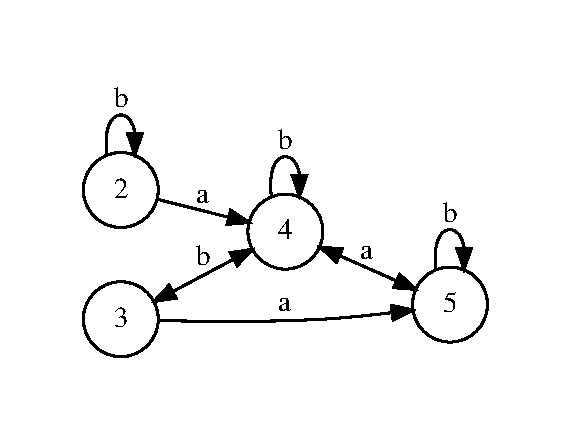
\includegraphics{pics/ch-pairs/tc-cayley-graph}
  \vspace{-4.0em}
  \caption[Todd--Coxeter example: right Cayley graph]
  {Right Cayley graph of $\pres{a, b}{ba=ab,\ b^2=b,\ a^3=ab,\ a^2b=a^2}$}
  \label{fig:tc-cayley-graph}
\end{figure}
It is worth noting that the columns of the table now give a right representation
of $S$.  That is, $S$ is isomorphic to the semigroup generated by the
transformations $\transV 34554$ and $\transV 22445$, as we can see from Theorem
\ref{thm:cayley-semigroups}: we have $(a)\phi = \transV 34554$ and
$(b)\phi = \transV 22445$, and these two transformations generate all the
elements of $\T_{S^1}$ apart from the identity.
\end{example}

We now consider another example, which shows that the Todd--Coxeter procedure can
take an unbounded length of time, even when the semigroup it computes is
relatively small.

\begin{example}
  \label{ex:tc-long}
  Let $\pres X R$ be the semigroup presentation
  $$\pres{a,b}{a^{100}=b,\ a=a^2}.$$
  By inspection we can see that any string $a^n$ is equal to $a$ by repeated
  application of the second relation, and therefore that $a = a^{100} = b$ by
  the first relation.  Hence any string in $X^+$ is equal to $a$, showing that
  $\pres X R$ defines the trivial
  semigroup.  However, if we apply the Todd--Coxeter procedure to this example,
  a table with 100 rows will need to be constructed before any coincidences are
  found, and 100 rows will need to be deleted before the algorithm terminates.

  The number $100$ in this example can be replaced by
  any arbitrarily large value; the presentation will still define the
  trivial semigroup, but computation time will be arbitrarily long.
  In this way, we can see that although the Todd--Coxeter algorithm is guaranteed
  to terminate in a finite number of steps when the input defines a finite
  semigroup, this number of steps is unbounded.
\end{example}

\subsubsection{Left, right, and two-sided congruences}
\label{sec:tc-l-r}
Next we will describe how to apply the given Todd--Coxeter method to
left, right and two-sided congruences.  The description of the Todd--Coxeter algorithm given
above is a method for finding the elements of the semigroup $S$ given by the
presentation $\pres X R$, and describing their multiplication.  More precisely,
the Todd--Coxeter algorithm produces a table in which each row represents one element
$s \in S^1$, each column represents one generator $x \in X$, and the cell in the
row of $s$ and the column of $x$ contains the row number of the element $sx$.
Hence its columns describe a right regular representation of $S$, as described
in Section \ref{sec:transformations}.  In the language of congruences, this is
equivalent to finding the classes of the trivial congruence $\Delta_S$ on the
semigroup $S$, or of the two-sided congruence $R^\sharp$ on the free semigroup
$X^+$.

The original problem we wanted to solve, as described in Section
\ref{sec:program-inputs}, is to find the classes of the congruence $\rho$
defined by a set of pairs $W \subset X^+ \times X^+$ over the semigroup defined
by $\pres X R$.  If we are considering
a two-sided congruence, we can simply apply the Todd--Coxeter method described
above to the semigroup presentation $\pres{X}{R,W}$, and the result will represent the
classes of $\rho$.  We call this method \textsc{ToddCoxeterTwoSided}, and give
pseudo-code for it in Algorithm \ref{alg:tc-twosided}.  Note that this
pseudo-code is precisely the same as \textsc{ToddCoxeter} in Algorithm
\ref{alg:tc}, except for the addition of lines 11--12 which trace all the
relations in $W$, before doing the same for those in $R$.

\begin{algorithm}
\caption{The \textsc{ToddCoxeterTwoSided} algorithm (for congruences)}
\label{alg:tc-twosided}
\index{ToddCoxeterTwoSided@\textsc{ToddCoxeterTwoSided}}
\begin{algorithmic}[1]
\Procedure{ToddCoxeterTwoSided}{$\pres X R$, $W$}
\State $n := 1$
\State $\mathbf{N} := \{1\}$
\State $\tau : \mathbf{N} \times X \to \mathbf{N} \cup \{0\}$
\For{$x \in X$}
  \State $(1, x)\tau := 0$
\EndFor
\State $e := 0$
\Repeat
  \State $e \gets e + 1$
  \If{$e \in \mathbf{N}$}
    \For{$(u,v) \in W$}
      \State \Call{Trace}{$e, u=v$}
    \EndFor
    \For{$(u,v) \in R$}
      \State \Call{Trace}{$e, u=v$}
    \EndFor
  \EndIf
\Until{$e = n$}  \Comment{There are no rows left to process}
\State \Return $(n, \mathbf{N}, \tau)$
\EndProcedure
\end{algorithmic}
\end{algorithm}

The correctness of the \textsc{ToddCoxeterTwoSided} algorithm is inherited from
the correctness of the \textsc{ToddCoxeter} algorithm, which is shown in, for
example, \cite{todd_coxeter_1936} and \cite{beetham_campbell_1976}.  What we
have precisely computed is the elements of the semigroup presented by
$\pres{X}{R,W}$, or in other words, the quotient semigroup $S / \rho$.  Each
class of $\rho$ is thus represented by one row in the resulting data structure.
Since this algorithm does not produce, for example, a list of all the elements
in a given class, we cannot yet say that we have ``computed'' the congruence in
the sense of the program outputs we specified in Section
\ref{sec:program-outputs}.  However, see the ``Computing program outputs''
section below for a description of the additional work required to produce all
the information we require about the congruence.

If we are considering a left or right congruence we
must alter the method slightly.  We shall now describe how to modify
the Todd--Coxeter algorithm to compute a table for the right congruence $\rho$ (see Algorithm
\ref{alg:tc-right} for pseudo-code).

Let $\pres X R$ and $W$ be as described in Section \ref{sec:program-inputs}, and
assume that $\rho$ is the right congruence they specify.  Since
$\pres X R$ specifies the semigroup over which $\rho$ is defined, we must trace
all the relations $R$ on every row in the table, as usual (lines 10--15).  This ensures that,
for a relation $(a,b) \in R$, we have $(i, a)\bar\tau = (i, b)\bar\tau$ for
every $i \in \mathbf{N}$, which is equivalent to the left congruence rule that
for any pair $(a,b) \in R$ we have $(sa, sb) \in \rho$ for every $s \in S$.
However, such a condition is not required for a right congruence, and so we do
not need to enforce the pairs from $W$ so strictly.  In fact, we only need to
trace the pairs from $W$ from row $1$, and not any other row, as we do in lines 7--8
of Algorithm \ref{alg:tc-right}.
The rest of the algorithm is the same as \textsc{ToddCoxeter} (Algorithm
\ref{alg:tc}), which is explained in detail above.

\begin{algorithm}
\caption{The \textsc{ToddCoxeterRight} algorithm (for right congruences)}
\label{alg:tc-right}
\index{ToddCoxeterRight@\textsc{ToddCoxeterRight}}
\begin{algorithmic}[1]
\Procedure{ToddCoxeterRight}{$\pres X R$, $W$}
\State $n := 1$
\State $\mathbf{N} := \{1\}$
\State $\tau : \mathbf{N} \times X \to \mathbf{N} \cup \{0\}$
\For{$x \in X$}
  \State $(1, x)\tau := 0$
\EndFor
\For{$(u,v) \in W$}
  \State \Call{Trace}{$1, u=v$}
\EndFor
\State $e := 0$
\Repeat
  \State $e \gets e + 1$
  \If{$e \in \mathbf{N}$}
    \For{$(u,v) \in R$}
      \State \Call{Trace}{$e, u=v$}
    \EndFor
  \EndIf
\Until{$e = n$}  \Comment{There are no rows left to process}
\State \Return $\tau$
\EndProcedure
\end{algorithmic}
\end{algorithm}

To see that this algorithm is correct, consider the following theorem.

\begin{theorem}
  Let $\pres X R$ and $W$ be as in Section \ref{sec:program-inputs} and $\rho$
  be the right congruence they specify.
  \textsc{ToddCoxeterRight($\pres X R$, $W$)} returns a table which describes the
  classes of $\rho$ (after the identity row $1$ is removed).
  \begin{proof}
    We may safely assume that the basic Todd--Coxeter algorithm is correct
    \cite{todd_coxeter_1936, beetham_campbell_1976} and therefore that
    \textsc{ToddCoxeterTwoSided($\pres X R$, $W$)} gives the correct answer for a
    two-sided congruence, since it is equivalent to running the Todd--Coxeter algorithm on the
    presentation $\pres{X}{R,W}$.  We must now consider how
    the \textsc{ToddCoxeterRight} algorithm differs from \textsc{ToddCoxeterTwoSided}, and
    prove that the resulting table does indeed define the right congruence
    $\rho$.

    \textsc{ToddCoxeterTwoSided} treats pairs from $R$ and pairs from $W$ in
    essentially the same way: each pair $(a,b)$ is traced starting at
    \textit{every} active row $e \in \mathbf{N}$, using
    \textsc{Trace}($e, a=b$).  \textsc{ToddCoxeterRight} follows this method for
    pairs in $R$, but traces pairs in $W$ only from row $1$.

    For a pair $(a,b) \in W$ we must certainly have $(a,b) \in \rho$.  Hence we
    run \textsc{Trace($1, a=b$)} on line 8 to ensure that $(1,a)\bar\tau = (1,b)\bar\tau$
    and therefore the row corresponding to $a$ is the same as the row
    corresponding to $b$.  However, we must not run \textsc{Trace($e, a=b$)} for
    any numbers $e$ higher than $1$, since this would be enforcing the
    \textit{left} congruence criterion
    (that $(sa, sb) \in \rho$ for all $s in S$), which does not apply to the
    \textit{right} congruence $\rho$.

    The right congruence criterion, that for any pair $(a,b) \in W$ we have
    $(as, bs) \in \rho$ for all $s \in S$, is automatically enforced without
    additional work, in the following way.  The words $as$ and $bs$ should be in
    the same congruence class of $\rho$ if and only if
    $(1, as)\bar\tau = (1, bs)\bar\tau$; but we already know that
    $(1, a)\bar\tau = (1, b)\bar\tau$, because it was enforced using
    $\textsc{Trace}$ on line 8, and so we have
    $$(1, as)\bar\tau
    = ((1, a)\bar\tau, s)\bar\tau
    = ((1, b)\bar\tau, s)
    = (1, bs)\bar\tau,$$
    which is enough to show that $(as, bs) \in \rho$ as required.
  \end{proof}
\end{theorem}

In summary, when computing a right congruence with the Todd--Coxeter algorithm, each relation
$u=v$ from $R$ must be applied to every single row $e \in \mathbf{N}$
(\textsc{Trace($e, u=v$)} as on line 14), while the relations from $W$ only need to be applied
to the identity row (\textsc{Trace($1, u=v$)} as on line 8).

If, instead of a right congruence, we are considering a left congruence, we may
apply the same method but reversing all multiplications.
This is shown in pseudo-code as \textsc{ToddCoxeterLeft} in Algorithm
\ref{alg:tc-left}.  The
row given by $(1, w_1 w_2 \ldots w_k)\bar\tau$ does not correspond to the word
$w_1 w_2 \ldots w_k$ but to the word $w_k w_{k-1} \ldots w_1$.  The words in
every relation in $R$ and $W$ should be reversed (lines 7 and 11) to make new
sets of relations $\bar R$ and $\bar W$, and then we should study the
right congruence defined by the resulting relations -- that is, the result of
$\textsc{ToddCoxeterRight}(\pres{X}{\bar R}, \bar W)$.  The Todd--Coxeter method
then works in exactly the same way as described above, but it should be
remembered on completion that the resulting table describes the semigroup and
congruence with left multiplication instead of right multiplication.

\begin{algorithm}
\caption{The \textsc{ToddCoxeterLeft} algorithm (for left congruences)}
\label{alg:tc-left}
\index{ToddCoxeterLeft@\textsc{ToddCoxeterLeft}}
\begin{algorithmic}[1]
\Procedure{ToddCoxeterLeft}{$\pres X R$, $W$}
\State $\bar R := \varnothing$
\State $\bar W := \varnothing$
\For{$(u,v) \in R$}
  \State Let $u = u_1 u_2 \ldots u_m$ \Comment{where each $u_i$ is in $X$}
  \State Let $v = v_1 v_2 \ldots v_n$ \Comment{where each $v_j$ is in $X$}
  \State $\bar R \gets \bar R \cup \{(u_m \ldots u_1, v_n \ldots v_1)\}$
\EndFor
\For{$(u,v) \in W$}
  \State Let $u = u_1 u_2 \ldots u_m$ \Comment{where each $u_i$ is in $X$}
  \State Let $v = v_1 v_2 \ldots v_n$ \Comment{where each $v_j$ is in $X$}
  \State $\bar W \gets \bar W \cup \{(u_m \ldots u_1, v_n \ldots v_1)\}$
\EndFor
\State \Return \Call{ToddCoxeterRight}{$\pres{X}{\bar R}, \bar W$}
\EndProcedure
\end{algorithmic}
\end{algorithm}

\begin{theorem}
  Let $\pres X R$ and $W$ be as in Section \ref{sec:program-inputs} and $\rho$
  be the left congruence they specify.
  \textsc{ToddCoxeterLeft($\pres X R$, $W$)} returns a table which describes the
  classes of $\rho$ (after the identity row $1$ is removed, and with respect to
  left multiplication).
  \begin{proof}
    For a word $w \in X^*$, let $\bar w$ be the reverse of that word, i.e.~if
    $w = w_1 w_2 \ldots w_n$ where $w_i \in X$ for all $i \in \{1 \ldots n\}$,
    then let $\bar w = w_n w_{n-1} \ldots w_1$.  Let $\bar R$ and $\bar W$ be
    produced from $R$ and $W$ as shown in Algorithm \ref{alg:tc-left}, by
    reversing all the words in all the pairs in each of the two sets.
    Note that for two words $u, v \in X^*$, $\overline{uv} = \bar v \bar u$, and
    that $\bar{\bar u} = u$.

    Let $S$ be the semigroup specified by the presentation $\pres X R$, and let
    $\bar S$ be the semigroup specified by the presentation $\pres{X}{\bar R}$.
    If $u$ and $v$ are two words in $X^+$, then $(u, v) \in R$ if and only if
    $(\bar u, \bar v) \in \bar R$.  This gives rise to a natural anti-isomorphism
    $\bar \cdot$ from $S$ to $\bar S$: if $w \in X^+$ represents some $s \in S$,
    then $\bar s$ is the element of $\bar S$ represented by $\bar w$.  This
    anti-isomorphism is the basis for \textsc{ToddCoxeterLeft}.

    Since $\rho$ is a left congruence, we have the rule that $(sa, sb) \in \rho$
    for every element $s \in S$ and every pair $(a,b) \in \rho$.  We define
    $$\bar\rho = \{(\bar a, \bar b) ~|~ (a,b) \in \rho\},$$
    a relation on $\bar S$.  The reflexivity, symmetry and transitivity of
    $\bar\rho$ follow from $\rho$.  But note that
    $(\overline{sa}, \overline{sb}) = (\bar a \bar s, \bar b \bar s) \in
    \bar\rho$
    for every $(\bar a, \bar b) \in \bar\rho$, and so $\bar\rho$ is a right
    congruence.  In fact, it is the right congruence generated by $\bar W$.

    Now when we call \textsc{ToddCoxeterRight}($\pres{X}{\bar R}, \bar W$) we
    know we are producing a table which represents $\bar\rho$.  We know that $S$
    is anti-isomorphic to $\bar S$, and that $(a,b) \in \rho$ if and only
    $(\bar a, \bar b) \in \bar\rho$, so the table can be used directly to
    describe $\rho$ itself.  We only need to take care to remember that all the
    multiplications shown by the Todd--Coxeter table $(n, \mathbf{N}, \tau)$ are
    actually left-multiplications.
  \end{proof}
\end{theorem}

\subsubsection{Computing program outputs}
\label{sec:tc-output}
So far we have described how the Todd--Coxeter procedure operates and the output
it produces.  However, on completion of \textsc{ToddCoxeterLeft} or
\textsc{Right} or \textsc{TwoSided}, it may not be immediately obvious how
information about the congruence can be retrieved from the resultant table.  In
this section we will explain how the output of these algorithms can be used to
produce the four program outputs (i) to (iv) required by Section
\ref{sec:program-outputs}.  Assume that we have taken inputs $X,R,W$ and applied
them to one of the three algorithms; let $\rho$ be the left, right, or two-sided
congruence described by these inputs, over the semigroup $S$.

Firstly, we require (i), an algorithm to determine whether a given pair $(x,y)$
of elements in the semigroup lies in $\rho$.  If $x$ and $y$ are elements of
$S$, then we can find words $w_x$ and $w_y$ over the alphabet $X$ which
represent them (see Section \ref{sec:program-inputs}).  We can then simply
compute \textsc{Trace}$(1, w_x)$ and \textsc{Trace}$(1, w_y)$, which will be
equal to each other if and only if $(x,y) \in \rho$.

For (ii), the number of congruence classes of $\rho$, we simply observe that
each congruence class is represented by one unique row in the Todd--Coxeter
table.  Each row corresponds to a single congruence class, except row 1 which
acts as an appended identity.  Hence the number of classes is equal to one less
than the number of rows in the table.

For (iii) we require an algorithm that takes an element $x$ and returns the
index of the congruence class to which it belongs.  As described above for (i),
we can simply take a word $w_x$ that represents $x$, and call
\textsc{Trace}$(1, w_x)$: the result is the index of the congruence class.

Finally, output (iv) is a list of the elements in each non-trivial congruence
class.  This is not so immediately available, but may still be computed if $S$
is finite.  Firstly, we require a list of the elements of $S$: if we have a
concrete representation, then this is given; if we have only a finite
presentation $\pres X R$ then \textsc{ToddCoxeter} can be called on the
presentation, and a representative word for each element can be found during
this run.  Once a list of elements is found, we can use \textsc{Trace} on each
element, as for (iii), to find which congruence class it lies in.  These results
can then be compiled, and singletons discarded, to produce the desired output.

Note that output (iv) cannot be produced using the Todd--Coxeter algorithm when $S$ is
infinite.  However, the pair orbit algorithm will succeed for infinite $S$, so
long as there are only finitely many elements in non-trivial classes.  See
Section \ref{sec:p} for more detail.

\subsubsection{Pre-filling the table}
\label{sec:tc-prefill}
\index{pre-fill}
In the ordinary Todd--Coxeter procedure as described above, we begin with just a
single row representing the empty word, and we add rows to represent the
different congruence classes as we go along, merging rows together if they are
found to describe the same congruence class.  However, in the case that we are
calculating a congruence over a concretely represented semigroup -- or indeed, over a finitely
presented semigroup on which the Todd--Coxeter algorithm has already been run -- we have certain
information which we can use to help us with our calculation.
We now describe how to use this information in a process called
\textit{pre-filling}, which represents new work in this area.

If we have such a semigroup $S$, then we can find a right Cayley graph $\Gamma$
for $S$ with respect to its generators $X$: if we have a concrete representation, then we can find
this graph using the Froidure--Pin algorithm (see Section \ref{sec:find-pres});
or if the Todd--Coxeter algorithm has been run on $S$, then the resulting table contains all
the information required for a right Cayley graph.  Either way, this graph tells us, for
each element $s \in S$ and each generator $x \in X$, the value of $s \cdot x$.
To \textbf{pre-fill} the table is to convert this Cayley graph into a
Todd--Coxeter table $(n, \mathbf{N}, \tau)$ with rows that represent the
elements of $S^1$, instead of starting with just a single row representing the
identity.  Then we only need to process the pairs in $W$ in order to calculate
the equivalence classes of $\rho$, and we do not need to use the pairs in $R$ at
all.  We now describe how this works in more detail, with pseudo-code in
Algorithm \ref{alg:tc-prefill}.

We initialise the table with $|S| + 1$ rows (line 2), all of them active (line
3), where row $1$ represents the identity as usual, and rows $2$ to $|S| + 1$
represent the elements of $S$.  We put these elements in some order such that
$S = \{s_1, s_2, \ldots, s_k\}$.  We now fill in the table, not with empty cells
as in previous Todd--Coxeter algorithms, but with the values we know they should
have according to the Cayley graph of $S$.

First, row $1$ represents the identity.  When we multiply the identity by a
generator $x$, we get $x$ itself.  Hence, for each $x \in X$, we fill in
$(1, x)\tau$ with the row that corresponds to $x$ -- that is, one more than the
position of $x$ in $S$ (lines 5--6).  Now, each of the rows beyond row $1$
corresponds to an element in $S$: row $i$ corresponds to the element $s_{i-1}$.
For each row $i$ and each generator $x$, we therefore need to fill the table in
with the row number of the element $s_{i-1} \cdot x$.  Hence we fill in
$(i, x)\tau$ with the row that corresponds to $s_{i-1} \cdot x$ -- that is, one
more than the position of $s_{i-1} \cdot x$ in $S$ (lines 7--8).

Recall the notation we defined in Section \ref{sec:program-inputs}: our
semigroup $S$ is presented by $\pres X R$, and we wish to calculate a congruence
$\rho$ defined by the generating pairs $W$.  \textbf{Pre-filling} the table with the
right Cayley graph as described in lines 1--8 above is equivalent to processing all the
relations $R$ and running the Todd--Coxeter algorithm to completion: we have a table which
describes the elements of $S$, or in other words, the classes of the trivial
congruence $\Delta_S$ on $S$.  In fact, the state of $(n, \mathbf{N}, \tau)$ at
the beginning of line 9 is the same as the output of
$\textsc{ToddCoxeter}(\pres X R)$, but may have taken much less time to compute.

Since we wish to calculate information about the classes of $\rho$, we now
have to consider the pairs $W$, and find out which $\Delta_S$-classes should be
combined to make $\rho$-classes.  Since there are no blanks in the table (i.e.~we never have
$(i,x)\tau=0$), we will never be forced to use the \textsc{Add} operation and
create new rows; the procedure from now on will simply be about tracing
relations from $W$ and combining rows together.  As we can see, the remainder of
the algorithm (lines 9--16) are the same as the final lines of
\textsc{ToddCoxeterTwoSided}, with the one difference that the two lines which
trace relations from $R$ have been removed -- these relations are now
unnecessary, since they are already incorporated into the table by prefilling
from the Cayley graph of $S$.  This is the main source of time-saving that
occurs in this algorithm, and is the key to its speed advantage over the
non-prefilled version (see Figures
\ref{fig:bench-trans-tc-1p-tccomp},
\ref{fig:bench-trans-tc-vp-tccomp} and
\ref{fig:bench-trans-tc-vp-right-bynrclasses} for performance benchmarks).

\begin{algorithm}
\caption{The \textsc{ToddCoxeterPrefill} algorithm}
\label{alg:tc-prefill}
\index{ToddCoxeterPrefill@\textsc{ToddCoxeterPrefill}}
\begin{algorithmic}[1]
\Require{$S = \{s_1, s_2, \ldots, s_k\}$ is a semigroup with its elements known in a defined order}
\Procedure{ToddCoxeterPrefill}{$\pres X R, W, S$}
\State $n := |S| + 1$
\State $\mathbf{N} := \{1 \ldots n\}$
\State $\tau : \mathbf{N} \times X \to \mathbf{N} \cup \{0\}$
\For{$x \in X$}
  \State $(1, x)\tau :=$ (position of $x$ in $S$) $+~1$
  \For{$i \in \{2 \ldots n\}$}
    \State $(i, x)\tau :=$ (position of $s_{i-1} \cdot x$ in $S$) $+~1$
  \EndFor
\EndFor

\State $e := 0$
\Repeat
  \State $e \gets e + 1$
  \If{$e \in \mathbf{N}$}
    \For{$(u,v) \in W$}
      \State \Call{Trace}{$e, u=v$}
    \EndFor
  \EndIf
\Until{$e = n$}  \Comment{There are no rows left to process}
\State \Return $(n, \mathbf{N}, \tau)$

\EndProcedure
\end{algorithmic}
\end{algorithm}

\begin{theorem}
  Let $\pres X R$ and $W$ be as in Section \ref{sec:program-inputs}, let $S$ be a
  semigroup presented by $\pres X R$, and assume we have a concrete
  representation for $S$.
  \textsc{ToddCoxeterPrefill}($\pres X R$, $W$, $S$) has output identical to
  \textsc{ToddCoxeterTwoSided}($\pres X R$, $W$), up to relabelling of the rows.
  \begin{proof}
    The only difference between \textsc{Prefill} and \textsc{TwoSided} is that
    \textsc{Prefill} initialises the Todd--Coxeter table with a right Cayley
    graph for $S$, while \textsc{TwoSided} computes one from scratch using $R$.

    % When, in line 11 of \textsc{TwoSided} (Algorithm \ref{alg:tc-twosided}), we
    % call \textsc{Trace} for a row $e$ and a relation $u=v$ from $R$, we are
    % simply forcing the equation $su = sv$ to hold, where $s$ is the element of
    % $S$ represented by row $e$.  But since $\pres X R$ is just a presentation
    % for $S$, there is no extra information it can give us which is not given by
    % $S$ itself.

    In lines 13 and 14 of \textsc{TwoSided} (Algorithm \ref{alg:tc-twosided}),
    we are doing the equivalent of the original \textsc{ToddCoxeter} algorithm,
    which produces a right Cayley graph for $S$.  Instead, in lines 2--8 of
    \textsc{Prefill} (Algorithm \ref{alg:tc-prefill}) we input a right Cayley
    graph for $S$ directly, without consulting $R$.  These two operations
    produce the same result -- a Todd--Coxeter table filled with a right Cayley
    graph for $S$ -- so it does not matter which method we use to do so.

    The only other part of the algorithm is to process the pairs in $W$,
    something which both algorithms do identically.  It might be noticed that in
    \textsc{TwoSided} this is done before the pairs in $R$.  Again, since the
    operation is equivalent to processing the presentation $\pres{X}{R,W}$, it
    does not matter in which order relations are processed.
  \end{proof}
\end{theorem}

It is worth noting that, unlike the other Todd--Coxeter algorithms described in
this thesis, \textsc{ToddCoxeterPrefill} is guaranteed to halt in finite time.
Since $X$ and $S$ are finite, the loops in lines 1--8 of the algorithm are
guaranteed to have a finite number of iterations.  In order to see that the
repeat-loop in lines 10--15 will also have a finite number of iterations,
observe that there are no blanks in the table -- that is, that there are no
values of $(i,x)$ such that $(i,x)\tau = 0$.  Since there are no blanks,
\textsc{Trace} can never cause a call to \textsc{Add}, and therefore the number
of rows $n$ will never go above $|S|+1$.  Hence the repeat-loop will go through
a maximum of $|S| + 1$ iterations, and since the for-loop inside iterates over a
finite set $W$, we are guaranteed completion in a finite number of steps.

\subsubsection{Implementation}

In the methods described above,
rows may be added to the table, and deleted from it.  A list must be kept of
rows which are in use; when a row is added, its position in the table should be
appended to this list at the end, and when a row is deleted it should be removed
from its position in the list and added to a list of ``free rows'' which can be
reused later.  The ``rows in use'' list is best implemented as a doubly-linked
list, so that single entries can be added and removed with as little processor
work as possible.

\subsection{Rewriting systems}
\label{sec:kb}

Another approach for solving the word problem in a finitely presented semigroup
is using rewriting systems.  Hence, given a semigroup $S$ with presentation
$\pres X R$ and a congruence $\rho$ over $S$ with generating pairs given by $W$
(see Section \ref{sec:program-inputs})
we may be able to find a rewriting system which converts any word $w \in X^+$ to
a canonical word representing the same element of $\pres X {R,\ W}$;
that is, a word representing a semigroup element in the same $\rho$-class as
the semigroup element of $S$ represented by $w$.

For ease of notation and understanding, this section will describe an algorithm
for the word problem on a finitely presented semigroup.  We understand that this
is the same as the problem of whether a given pair of words represent semigroup
elements related to each other by a two-sided congruence $\rho$.  The current
implementation of this method in \libsemigroups{} does not include left and
right congruences as an option (but see Section \ref{sec:kb-l-r}).

In order
to describe the process, we must first explain some background theory.  A full
description of these ideas can be found in \cite[Section 12.2]{cgt}.  Note that
we shall again consider monoid presentations instead of semigroup presentations,
since it is easy to change between the two by appending or removing an identity
(the empty string $\varepsilon$).

\begin{definition}
  \label{def:rws}
  \index{rewriting system}
  \nomenclature[Rb]{$\rws$}{Rewriting system}
  Let $X$ be an alphabet.  A \textbf{rewriting system} $\rws$ on $X^*$ is a set
  of ordered pairs $(u,v)$ where $u, v \in X^*$.
\end{definition}

A pair $(u,v) \in \rws$ is called a \textit{rule}, and can be viewed as
an operation which transforms an occurrence of $u$ in a word into an occurrence
of $v$.
For this section, we will assume that $\rws$ is finite.
A rewriting system $\rws$ extends to relations
$\to_\rws$, $\tostar_\rws$, and $\lrstar_\rws$
which describe how words are rewritten, and which are defined as follows.

\nomenclature[->R]{$\to_\rws$}{Rewriting system operation}
\nomenclature[->R*]{$\tostar_\rws$}{Reflexive transitive closure of rewriting system operation}
\nomenclature[->R*<]{$\lrstar_\rws$}{Equivalence of rewriting system operation}
Let $u, v \in X^*$ and let $\rws$ be a rewriting system.
We write $u \to_\rws v$ if there exist $(w_1, w_2) \in \rws$ and
$s, t \in X^*$ such that $u=sw_1t$ and $v=sw_2t$.
That is, $u \to_\rws v$ if a rule rewrites a contiguous subword of $u$ to turn
$u$ into $v$.  The relation $\tostar_\rws$ is simply the reflexive transitive
closure of $\to_\rws$; that is, $u \tostar_\rws v$ if and only if $u = v$ or
$$u = u_0 \to_\rws u_1 \to_\rws \cdots \to_\rws u_n = v,$$
for some $u_0, \ldots, u_n \in X^*$.
Finally, $\lrstar_\rws$ is the symmetric closure of
$\tostar_\rws$.  It is easy to see that $\lrstar_\rws$ is an equivalence
relation whose classes we may write as $[w]_\rws$.
Where there is no chance of ambiguity, we omit the subscript in these
operations, just writing $\to$, $\tostar$ and $\lrstar$.

This definition of a rewriting system does not guarantee that a word can be
rewritten in a useful way.  A rewriting system could allow an endless loop of
rewriting; for example, a system over the alphabet $\{a,b\}$ could contain rules
$(aa,b)$ and $(b,aa)$ which would allow the rewrite sequence
$$aa \to b \to aa \to b \to aa \to b \to aa \to \cdots$$
to go on forever.  It could also be possible to rewrite one word in
two different ways; for example, a system over the alphabet $\{a,b,c\}$ could
contain rules $(aa,b)$ and $(aa,c)$.

In order to solve the word problem for a semigroup, we require a
rewriting system with certain properties.  We will describe these properties,
and then explain how to produce a rewriting system which satisfies them.

\begin{definition}
  \label{def:irreducible}
  \index{irreducible}
  A string $u \in X^*$ is $\rws$-\textbf{irreducible} if there is no
  string $v \in X^*$ such that $u \to v$; that is, $u$ cannot be rewritten by
  any rule in $\rws$.  \cite[Def~12.13]{cgt}
\end{definition}

\begin{definition}
  \label{def:terminating}
  \index{terminating}
  A rewriting system is \textbf{terminating} if there is no infinite chain of
  words $u_1, u_2, \ldots \in X^*$ such that $u_i \to u_{i+1}$ for all $i > 0$.
\end{definition}

If a rewriting system is terminating, this is good news computationally.  It
means that any word can be transformed by rules only a finite number of times
before it reaches an irreducible state, so the task of finding an irreducible
form of a word is guaranteed to be achievable in finite time.  But note that we
can still only talk about \textit{an} irreducible word, not \textit{the}
irreducible word.  We could still have a word $u \in X^*$ and irreducible words
$v, w \in X^*$ such that $u \tostar v$ and $u \tostar w$ but $v \neq w$.
To avoid this, we must ensure that the system is \textit{confluent}, as follows.

\begin{definition}
  \label{def:confluent}
  \index{confluent}
  A rewriting system is \textbf{confluent} if, for any words $u,v_1,v_2 \in X^*$
  such that $u \tostar v_1$ and $u \tostar v_2$, there exists a word $w \in X^*$
  such that $v_1 \tostar w$ and $v_2 \tostar w$.
\end{definition}

The intuition behind this definition is that, as the name suggests, different
paths ``flow together''.  The result is that, in a confluent terminating
rewriting system, rules can be applied to a word in any order, and a canonical
irreducible word will be found in a finite number of steps.
% If $\rws$ is
% a confluent terminating rewriting system, then let us write $(w)f_\rws$
% or $(w)f$ for the unique irreducible word which $w$ can be written to.  Let
% $[w]_\rws$ or $[w]$ be the set of all words $u \in X^*$ such that
% $u \tostar (w)f$.

Another definition will help us to determine whether a rewriting system is
confluent: \textit{local confluence}.  This is a weaker condition than
confluence, but the two are strongly linked by Lemma \ref{lem:newman}.

\begin{definition}
  \label{def:locally-confluent}
  \index{locally confluent}
  A rewriting system is \textbf{locally confluent} if, for any words
  $u,v_1,v_2 \in X^*$ such that $u \to v_1$ and $u \to v_2$, there exists a word
  $w \in X^*$ such that $v_1 \tostar w$ and $v_2 \tostar w$.
\end{definition}

\begin{lemma}[Newman's diamond lemma {\cite[Lemma 12.15]{cgt}}]
  \label{lem:newman}
  A terminating rewriting system is confluent if and only if it is locally
  confluent.
\end{lemma}

Lemma \ref{lem:newman} gives us an idea of how to check computationally whether
a system is confluent: rather than checking every possible transitive rewriting
of a word (its neighbours under $\tostar$), it suffices to check a word's
immediate children (its neighbours under $\to$).  This lemma will help us later,
with Theorem \ref{thm:knuth-bendix} and the Knuth--Bendix procedure.

We can now see an application of rewriting systems to the word problem in a
finitely presented monoid.  Indeed, given an alphabet $X$ and a rewriting system
$\rws$, the quotient monoid $X^* / \lrstar_\rws$ is described by the
monoid presentation $\pres{X}{\rws}$.  Hence, given a monoid $M$ with a
presentation $\pres X R$, if there is a confluent terminating rewriting system
$\rws$ such that the word equality relation $=_M$ is the same as the
relation $\lrstar_\rws$, then the word problem can be solved
simply by rewriting two words using $\rws$ until their irreducible
representatives are found, and then comparing them.  The only difficulty is in
finding a rewriting system which is confluent and terminating -- but we can find
one, by starting with the set of relations $R$, and then using the Knuth--Bendix
completion algorithm.

Let $M$ be a monoid with finite presentation $\pres X R$.  We start with no
rules in our rewriting system, $\rws = \varnothing$, and we begin to add
relations from $R$.  However, in order to ensure our system is
\textit{terminating}, we must reorder each relation to ensure we do not create
any loops.  For this purpose, we define a total ordering $\leq$ on $X^*$ and
reorder each relation so that a rule $(u, v)$ has the property that $u > v$.
Our chosen ordering $\leq$ must be a \index{reduction ordering}
\textit{reduction ordering}, meaning that if we have $u \leq v$ then we must
also have $wux \leq wvx$ for all $w,x \in X^*$ \cite[\S12.2]{cgt}.  For our
purposes, it will suffice to use the \index{shortlex ordering} \textit{shortlex
  ordering}: $u < v$ if and only if $u$ is shorter than $v$ or they have equal
length and $u$ is less than $v$ lexicographically.  Hence the first few words
over the alphabet $\{a, b\}$ are
$$\varepsilon < a < b < aa < ab < ba < bb < aaa < aab < aba < \cdots$$
Note that this requires a well-understood total order on the alphabet $X$
itself.  Another possible reduction ordering is \textit{wreath product ordering}
\cite[\S2.1]{sims}, which has a particular application to polycyclic groups;
however, this has no particular advantage when applied to semigroups, so the
simpler shortlex ordering is preferable.

The use of a reduction ordering justifies the use of the words ``reducible'' and
``irreducible'' -- words are always replaced with lesser words.  We must ensure,
at all points during the algorithm, that every rule $(u,v) \in \rws$ satisfies
$u > v$.

\begin{example}[Exercise 3.1 in {\cite[\S2.3]{sims}}]
  \label{ex:rws}
  Let $X = \{a,b\}$, and let $\rws$ be a rewriting system on $X^*$ given by
  $$\rws = \Big\{
  \big(a^5, \varepsilon\big),
  \ \big(b^5, \varepsilon\big),
  \ \big(b^4a^4, (ab)^4\big),
  \ \big((ba)^4, a^4b^4\big)
  \Big\}.$$
  We can apply any sequence of these rules to any word we wish.  For example, we
  can rewrite the word $b^5a^6$ using the last two rules as follows:
  $$b^5a^6
  = b\underline{bbbbaaaa}aa
  \to_\rws ba\underline{babababa}a
  \to_\rws baaaaabbbba.$$
  Hence $b^5a^6 \tostar_\rws ba^5b^4a$.  Alternatively we could rewrite it using
  the first two rules:
  $$b^5a^6
  \to_\rws \varepsilon a^6
  = a^5a
  \to_\rws \varepsilon a
  = a.$$
  Hence $b^5a^6 \tostar_\rws a$.  Using both these results together with
  transitivity, we have $a \lrstar_\rws ba^5b^4a$.

  Let us consider the shortlex ordering described above.  The first two rules in
  $\rws$ shorten a word by 5 characters, and the last two rules replace a
  subword of length 8 beginning with $b$ by one beginning with $a$.  Hence all
  four rules $(u,v)$ have $u > v$ with respect to shortlex ordering.  Hence
  $\rws$ is a terminating rewriting system.
\end{example}

Once each relation from $R$ is added -- possibly reordered -- to $\rws$, we
will have a terminating rewriting system such that
$X^* / \lrstar_\rws\ = \pres X R$, as required.  It only remains to add
rules to $\rws$ to make it confluent, without altering the relation
$\lrstar$.  This is where we use the Knuth--Bendix completion process.

\index{Knuth--Bendix}
First described by Knuth and Bendix in \cite{knuth_bendix}, the completion
process adds rules to $\rws$ by finding and resolving
\textit{critical pairs}.  A critical pair is a pair of rules $(u_1, v_1)$ and
$(u_2, v_2)$ from $\rws$ such that $u_1$ and $u_2$ overlap in a certain way.
They are defined as follows, as in \cite[Lemma 12.17]{cgt}.

\begin{definition}
  \label{def:critical-pair}
  \index{critical pair}
  Let $\rws$ be a terminating rewriting system over an alphabet $X^*$.  A
  \textbf{critical pair} is a pair of rules $(u_1, v_1)$ and $(u_2, v_2)$ in
  $\rws$ such that one of the following is true:
  \begin{enumerate}[\rm(i)]
  \item $u_1 = rs$ and $u_2 = st$ with $r,s,t \in X^*$ and
    $s \neq \varepsilon$;
    %then $rst \to v_1t$ and $rst \to rv_2$, so
    %$(v_1t, rv_2)$ is a critical pair.
  \item $u_1 = ru_2t$ for some $r,t \in X^*$ and $u_2 \neq \varepsilon$.
    %then $u_1 \to v_1$ and $u_1 \to rv_2t$, so $(v_1, rv_2t)$ is a critical
    %pair.
  \end{enumerate}
\end{definition}

A critical pair results in a choice when applying rewriting rules, which leads
to different results depending on which rule is applied.  A critical pair of
type (i) allows us to rewrite $rst$ to either $v_1t$ or $rv_2$, depending on
which rule is applied; and a critical pair of type (ii) allows us to rewrite
$u_1$ to either $v_1$ or $rv_2t$, depending on which rule is applied.  In order
for $\rws$ to be confluent, we have to ensure that whichever option is chosen, a
word is still rewritten to a fixed word later on.  This notion is made precise
in the following theorem, which is key to the Knuth--Bendix completion process.

\begin{theorem}[{\cite[Lemma 12.17]{cgt}}]
  \label{thm:knuth-bendix}
  A terminating rewriting system $\rws$ over $X$ is confluent if and only if,
  for each critical pair of rules $(u_1, v_1)$ and $(u_2, v_2)$, the following
  hold:
  \begin{enumerate}[\rm(i)]
  \item if it is a critical pair of type (i), there exists some word $w \in X^*$
    such that $v_1t \tostar_\rws w$ and $rv_2 \tostar_\rws w$;
  \item if it is a critical pair of type (ii), there exists some word
    $w \in X^*$ such that $v_1 \tostar_\rws w$ and $rv_2t \tostar_\rws w$.
  \end{enumerate}
\end{theorem}

Now we have all the concepts required to describe the Knuth--Bendix completion
process.  The process searches through rules in $\rws$ looking for critical
pairs; when a critical pair is found which does not satisfy the
condition stated in Theorem \ref{thm:knuth-bendix}, an appropriate word $w$ is
chosen and the rules required in Theorem \ref{thm:knuth-bendix} are
added to $\rws$ in order to ensure confluence.

Though, as mentioned in Section \ref{sec:computation-decidability}, the word problem for a
semigroup presentation is undecidable in general, we do have a result about the
Knuth--Bendix process which ensures completion in some cases.

\begin{theorem}
  \label{thm:kb-halt}
  Let $S$ be a semigroup with a finite presentation $\pres X R$, and let $\rws$
  be the rewriting system produced from $R$ by applying a shortlex ordering to
  all pairs, as described above.

  If $S$ is finite, then the Knuth--Bendix process applied to $\rws$ will
  eventually halt with a finite, confluent and terminating set of rules.

  \begin{proof}
    Let $u,v \in X^*$.  We know that $u \lrstar_\rws v$ if and only if $u$ and
    $v$ describe the same element of $S$.  In particular, if $S$ is finite, then
    the $\lrstar_\rws$ relation will have finitely many classes -- one for each
    element of $S$.  Finally, \cite[Corollary 12.21]{cgt} tells us that if the
    Knuth--Bendix algorithm is run on any rewriting system $R$ such that
    $\lrstar_R$ has only finitely many classes, it will halt with a finite,
    confluent and terminating set of rules.  This applies to our rewriting
    system $\rws$, and so we have the result we need.
  \end{proof}
\end{theorem}

Let us consider an example of each of the two types of critical pair in
Definition \ref{def:critical-pair}.

\begin{example}
  Let $X=\{a,b,c\}$, and let $\rws$ be a rewriting system on $X$, containing
  two rules $(ab, c)$ and $(bb, a)$.  Here the word $abb$ could be
  rewritten by either rule: $abb = (ab)b \to cb$, but also
  $abb = a(bb) \to aa$.  Hence $(cb, aa)$ is a critical pair of type (i).

  If there exists some $w \in X^*$ such that $cb \tostar w$ and $aa \tostar w$,
  then confluence is not violated; otherwise, we must add a new rule to $\rws$
  to make sure confluence holds.  The Knuth--Bendix process adds the rule
  $(cb, aa)$, since $aa < cb$ in our shortlex order.  Now Theorem
  \ref{thm:knuth-bendix} is satisfied.
\end{example}

\begin{example}
  Let $X=\{a,b,c\}$ and let $\rws$ be a rewriting system on $X$ with rules
  $(abc, c)$ and $(b, a)$.  The word $abc$ can now be written by either rule,
  $abc \to c$ or $abc \to aac$.  Hence $(c, aac)$ is a critical pair of type
  (ii).

  Again, if there are other rules allowing both words to be rewritten to a word
  $w \in X^*$, then no rules need to be added; if however there are no such
  rules, we must add $(aac, c)$ to ensure the theorem is satisfied, and
  confluence can be guaranteed.
\end{example}

The Knuth--Bendix completion process consists of searching for these critical
pairs and adding rules where necessary.  For a more detailed description of
precisely how these tasks are done, see \cite[\S 2.6]{sims}.

A large part of the computational work involved in the Knuth--Bendix process
consists of rewriting words using rules from $\rws$.  If the rewriting system is
confluent and terminating, then the rules can be applied in any order and an
irreducible word will eventually be reached.  However, the order in which the
rules are applied can have a great effect on the overall runtime of the
algorithm.  In Algorithm \ref{alg:rewrite} we present one possible strategy,
known as \textit{rewriting from the left}, which is based on the
REWRITE\texttt{\char`_}FROM\texttt{\char`_}LEFT procedure described in
\cite[\S2.4]{sims}, where the issues of termination and correctness are
addressed formally.  The algorithm takes two arguments -- a word $u$ and a terminating
rewriting system $\rws$ -- and returns the irreducible word produced from $u$ by
applying rules in $\rws$.

The \textsc{Rewrite} algorithm starts with the original word $u$, and an empty
word $v$.  We enter a loop that constitutes the rest of the algorithm.  On each
iteration, we start by removing the first character from $u$ and putting it onto
the end of $v$ (lines 4--6).  Next we go through each rule $p \to q$ in $\rws$
(line 7) and attempt to apply it to a suffix of $v$ -- that is, we check whether
$v$ ends in $p$ (line 8).  If we find a rule $p \to q$ such that $v$ does end in
$p$, then we remove the occurrence of $p$ from the end of $v$ (line 9) and we
add the rewritten version $q$ to the beginning of $u$ (line 10) for further
processing in a later iteration of the repeat-loop.  After finding just one of
these rules to apply, we stop going through rules (line 11) and if appropriate,
go back to the beginning of the repeat-loop (line 11).  When the whole word has
been processed and $u$ is therefore empty (which will happen in finite time so
long as $\rws$ is terminating and confluent) we return $v$, which is the
irreducible result of $u$ after a series of rules from $\rws$ have been applied.

\begin{algorithm}
\caption{The \textsc{Rewrite} algorithm}
\label{alg:rewrite}
\index{Rewrite@\textsc{Rewrite}}
\begin{algorithmic}[1]
\Procedure{Rewrite}{$u, \rws$}
\State $v := \varepsilon$
\While{$u \neq \varepsilon$}
  \State Let $u_1$ be the first character of $u$
  \State $v \gets v u_1$
  \State Remove the first character of $u$
  \For{$(p,q) \in \rws$}
    \If{$v = rp$ for some $r \in X^*$}
      \State $v \gets r$
      \State $u \gets qu$
      \State \Break
    \EndIf
  \EndFor
\EndWhile
\State \Return $v$
\EndProcedure
\end{algorithmic}
\end{algorithm}

It should be noted that, like the Todd--Coxeter procedure, there is no guarantee
that the Knuth--Bendix algorithm will complete in a finite time unless the presentation
$\pres X R$ is known to define a finite semigroup.  More rules may be added continually, which
themselves need to be checked for critical pairs, without a complete set ever
being found.  It may also be that a confluent terminating rewriting system will
eventually be found, but not for a very long time -- and it is never known in
advance whether the process is going to terminate.  However, this process has
one clear advantage over the Todd--Coxeter algorithm, which is that it may complete even when
the monoid $\pres X R$ is infinite, so long as the set of rules in the rewriting
system is finite (see Example \ref{ex:bicyclic}).  This is a strong argument in
favour of trying the Knuth--Bendix process along with other methods.  The
Knuth--Bendix process as currently implemented cannot be used for left or right
congruences, an area where the Todd--Coxeter algorithm has a clear advantage (but again, see
Section \ref{sec:kb-l-r}).

We give an example of a rewriting system which solves the word problem for an
infinite monoid:

\begin{example}
  \label{ex:bicyclic}
  The \textit{bicyclic monoid} $B = \pres{b,c}{bc=\varepsilon}$ trivially admits
  a rewriting system $\{(bc, \varepsilon)\}$.  Using this, any element can be
  rewritten in a finite number of steps to an irreducible word of the form
  $c^ib^j$.  There is only one rule in the rewriting system.  Since it reduces
  words by the \textit{short-lex} ordering, the system is terminating; and since
  there are no critical pairs, the system is confluent by Theorem
  \ref{thm:knuth-bendix}.
\end{example}

\subsubsection{Computing program outputs}
\label{sec:kb-output}
We have shown how the inputs $X$, $R$ and $W$ can be used as inputs to the
Knuth--Bendix algorithm in order to produce a rewriting system.  However, we
have not explicitly stated how this can be used to produce the information we
require about the congruence in question, in the sense of the four program
outputs in Section \ref{sec:program-outputs}.  We will now consider each of
these outputs in turn, and explain how the rewriting system $\rws$ can be used
to produce them.  Let $X$, $R$ and $W$ be as described earlier, let $S$ be the
semigroup in question, and let $\rho$ be the congruence we are computing.

For (i) we require an algorithm to determine whether a given pair $(x,y)$ is in
$\rho$.  This is the simplest of the four: we take two words $w_x$ and $w_y$
over the alphabet $X$, which represent $x$ and $y$ respectively, and we rewrite
them both using $\rws$.  The pair $(x,y)$ is in the congruence if and only if
the two words rewrite to the same word.

For (ii) we require the number of classes the congruence has.  As just
mentioned, an element's class is defined by the word produced by rewriting it
with $\rws$; hence, the number of classes is equal to the number of different
words to which words can be rewritten.  If $S$ is finite, this number can be
found by taking a word that represents each element of $S$, rewriting it with
$\rws$, and calculating the number of distinct words computed.  However, if $S$
is infinite, we do not have such a method available, and we cannot return a
number in this case.  Note that there could still be a finite number of classes,
in which case the Todd--Coxeter algorithm could return an answer (see
``Computing program outputs'' in Section \ref{sec:tc-output}).

For (iii) we require an algorithm \textsc{ClassNo} that takes an element $x$ and
returns the index of the congruence class to which it belongs.  That is, it
should return a positive integer for any element, and it should have the same
output for elements $x$ and $y$ if and only if $(x,y) \in \rho$.  In
\libsemigroups{} we take an approach which creates indices for classes as calls
are made to the algorithm.  We start with an empty list $L$.  When
\textsc{ClassNo}$(x)$ is called, the algorithm takes a word representing $x$,
and rewrites it to some word $w$ using the rewriting system $\rws$.  If $w$ is
in $L$, then the algorithm returns its position in the list; if not, then the
algorithm adds it to the end of $L$, and returns its new position.  This gives
\textsc{ClassNo} the required behaviour, but it is important to note that the
outputs depend on the order in which past calls were made.  In two different
program sessions, in which calls were made in a different order, different
numbers would be returned.  In this sense, \textsc{ClassNo} is not canonical.

Finally, for (iv), we wish for a list of the elements in each non-trivial
congruence class.  If $S$ is finite and we have a list of its elements, we can
use (iii) and apply \textsc{ClassNo} to each element, to find out which elements
lie in which class.  However, if $S$ is infinite, no such method is available,
and we would have to rely on the pair orbit algorithm to produce the answer.

Note that outputs (ii) and (iv) require a list of the elements of $S$, which
might not be immediately available at the end of the Knuth--Bendix algorithm.
If we have a concrete representation for $S$, then we do have a list of all the
elements of S.  However, if we only have a finite presentation for $S$, then we
would need to run another algorithm such as the Todd--Coxeter algorithm on
$\pres X R$ in order to find a list of its elements.

\section{Running in parallel}
\label{sec:running-in-parallel}

Now that we have described the various individual algorithms for computing with
congruences, we can describe the overall parallel method which ties all these
algorithms together.

The basic principle is not complicated: run all the described algorithms
simultaneously, and whenever one of the algorithms finds an answer, kill all the
other algorithms and return the answer that was given.  However, the precise
details depend on whether we have a concrete representation or a finite
presentation, as well as whether we are considering a left, right or two-sided
congruence.  Table \ref{tab:running-in-parallel} shows which algorithms are run
in which cases.  A tick (\cmark) denotes that the algorithm is used, a cross
(\xmark) denotes that it cannot be used, and a tilde ($\sim$) denotes that the
algorithm could be applied in principle, but is so rarely the fastest option that in practice
it is not worth including.

\begin{table}[ht]
  \centering
  \renewcommand{\arraystretch}{1.3}
  \begin{tabular}{| c | r | c | c | c | c |}
    \hline
    Type & Side & TC & TC (pre-fill) & P & KB \\
    \hline
    \multirow{2}{*}{Concrete} & Two-sided & \cmark & \cmark & $\sim$ & $\sim$ \\
    \cline{2-6}
         & Left/right & \cmark & \cmark & $\sim$ & \xmark \\
    \hline
    \multirow{2}{*}{FP} & Two-sided & \cmark & \xmark & \cmark & \cmark \\
    \cline{2-6}
         & Left/right & \cmark & \xmark & \cmark & \xmark \\
    \hline
  \end{tabular}
  \renewcommand{\arraystretch}{0.7}
  \caption{The algorithms that are used in various cases}
  \label{tab:running-in-parallel}
\end{table}

The positions in the table marked with a tilde are chosen based on extensive
benchmarking tests with \libsemigroups{}, which can be seen in detail in
Section \ref{sec:benchmarking}.  It is true that in certain examples these
algorithms will complete faster than the others; however, so few of these
examples have been encountered that it seems more desirable to eliminate the
setup cost and overheads for these algorithms by omitting them entirely, since
in the vast majority of cases this will speed things up.

It should be noted that any one of these algorithms might be able to return an
answer before its respective data structure has been completely evaluated.  For
instance, if we are running the Todd--Coxeter algorithm in order to decide whether two words
$u$ and $v$ are congruent, we can at any time check whether
$(1,u)\bar\tau = (1,v)\bar\tau$: if this equality holds, then the two words lie
in the same congruence class, and since a class is never split in two by the
Todd--Coxeter algorithm, an answer of ``true'' can be returned immediately,
without any need to run the algorithm until a complete table is found.  If, on
the other hand, $(1,u)\bar\tau \neq (1,v)\bar\tau$, then we cannot return an
answer: it might be that the words genuinely lie in different congruence
classes, or it might be that a coincidence between their rows will be found in
the future.  An answer of ``false'' can therefore not be returned until
the Todd--Coxeter algorithm is run to completion.

A similar condition is true for both the Knuth--Bendix algorithm and pair orbit enumeration.
Imagine we have a rewriting system $\rws$ halfway through a run of the Knuth--Bendix algorithm;
if two words $u$ and $v$ rewrite to the same word under $\rws$, then we can
return ``true'' immediately, but if they do not, then it might be that
the Knuth--Bendix algorithm will add rules to $\rws$ later which will cause $u$ and $v$ to
rewrite to the same word.  Pair orbit enumeration has this condition even more
obviously: more and more pairs are found, and the pair we are looking for can
turn up at any time.

In an implementation of this parallel method, it is therefore prudent to
have a periodic check to see whether a desired pair is present, and return
immediately if it is.  This check could be done by each individual algorithm
every few hundred operations, or on a timer every few milliseconds.  In this
way, operations can quickly return desired results, even if it would take them a
very long time (or even an infinite length of time) to run to completion.

% \begin{algorithm}
% \caption{Determining whether $x$ and $y$ represent the same class of the
%   congruence on $\pres X R$ generated by $W$ (finitely presented)}
% \label{alg:pair-in-cong-fp}
% \begin{algorithmic}[1]
% \Require $x,y \in X^+$
% \Procedure{PairInCong}{$\pres{X}{R}, W, (x,y)$}
% \State Run \Call{ToddCoxeter}{$\pres{X}{R,W}$}
%        until completion or until $x~\rho~y$
% \State $\rws := R \cup W$
% \State Run \Call{KnuthBendix}{$\rws$}
%        until completion or until $x~\rho~y$
% \EndProcedure
% \end{algorithmic}
% \end{algorithm}

% \begin{algorithm}
% \caption{Determining whether $(x,y)$ lies in $\mathbf{R}^\sharp$}
% \label{alg:pair-in-cong-concrete}
% \begin{algorithmic}[1]
% \Procedure{PairInCong}{$\pres{X}{R}, W, (x,y)$}
% \Require $x,y \in X^+$
% \State Run \Call{ToddCoxeter}{$\pres{X}{R,W}$}
%        until completion or until $x~\rho~y$
% \State Run \Call{ToddCoxeterPrefill}{$\pres{X}{R}, W, S$}
%        until completion or until $x~\rho~y$
% \EndProcedure
% \end{algorithmic}
% \end{algorithm}

% TODO? \section{Implementation}

\section{Benchmarking}
\label{sec:benchmarking}

The approach described in this chapter was implemented in the C++ programming
language in \libsemigroups{} \cite{libsemigroups}, and this allows us to
run benchmarking tests to analyse the performance of the different algorithms,
compared to each other and compared to existing programs.  In this section we
provide some examples of such tests.

\subsection{Examples}
Firstly, it will be helpful to examine a few examples of problems which can be
solved by the different algorithms, and to compare the types of problems in
which each algorithm is most effective.  These examples were implemented in the
benchmarking section of \libsemigroups{}, and their performance was tested
with various algorithms.

\begin{example}
  \label{ex:good-tc}
  \nomenclature[PBn]{$\PBR_n$}{Full PBR monoid}
  Consider $\PBR_2$, the full PBR monoid of degree $2$ -- this is a special type
  of diagram monoid based on directed graphs, and is explained in detail in
  \cite[\S2.1]{diagram_semigroups}.  It has $65536$ elements and is therefore
  large enough to require significant processing time when considering its
  congruences.  We take a set of pairs which we know will generate a two-sided
  congruence equal to the universal congruence, and we ask \libsemigroups{} for
  the number of congruence classes, using the simple Todd--Coxeter algorithm in one case and
  the pre-filled Todd--Coxeter algorithm in the other.

  On average, the simple Todd--Coxeter algorithm returns an answer in 724 milliseconds, while
  the pre-filled version requires an average of 3057 milliseconds, more than 4
  times as long.  This difference can be explained by the structure
  of the table at completion: a single row representing the one congruence
  class.  In the pre-fill case, a coset table must be constructed with 65536
  rows, only to have all but one row deleted.  In the simple case,
  the number of rows may stay very small throughout the procedure, drastically
  reducing the amount of work which needs to be done.
\end{example}

\begin{example}
  \label{ex:good-tc-prefill}
  The virtue of the pre-filled Todd--Coxeter algorithm is shown by a different congruence on
  $\PBR_2$.  A much smaller set of generating pairs gives rise to a two-sided congruence
  $\rho$ with 19009 congruence classes, in contrast to the universal congruence
  which has only one.  On average, the simple Todd--Coxeter algorithm returns in around 128
  seconds, while the pre-filled version completes in under 12 seconds, a tenfold
  increase in speed.  This disparity can be explained by the large number of
  rows which must be in the table on completion: the simple algorithm has to
  compute a large amount of information from relations, and add rows one by one,
  while the pre-filled algorithm begins the process with much of the table's
  information already known, and only has to combine rows which coincide.
\end{example}

The two examples above show the difference in speed between two algorithms.  We
now consider an example where certain algorithms will never terminate, but
others complete quickly.  This is an even greater justification for the parallel
use of a variety of algorithms.

\begin{example}
  \label{ex:good-kbfp}
  Consider the semigroup $S$ defined by the semigroup presentation
  $$\pres{a,b}{a^3=a,\ ab=ba}.$$  We define $\rho$ to be the two-sided congruence on $S$
  generated by the single pair $(a, a^2)$.  Since each word of the form $b^i$
  represents a different element of $S$, and a different class of $\rho$, we can
  conclude that $S$ is infinite and $\rho$ has an infinite number of congruence
  classes.  A test asks whether $(ab^{20}, a^2b^{20})$ is a pair in $\rho$.  The
  Todd--Coxeter methods would never complete, since they require a separate row
  for each congruence class and therefore an infinite amount of memory.
  However, the Knuth--Bendix method is able to answer the question very quickly,
  since it is not restricted to finite objects.
\end{example}

% A specific utility of the Knuth--Bendix algorithm with pair orbit enumeration (\texttt{kbp}) is
% the ability to return a congruence's \textit{non-trivial congruence classes},
% which in some cases cannot be determined by any of the other algorithms.
% Consider the following example.

% \begin{example}
%   \label{ex:good-kbp}

%   Let $S$ be the semigroup defined by the presentation
%   $$\pres{a,b,c}{b^7=b,\ c^5=c,\ bc^2ba=bc^2b,\ bc^2bc=bc^2b,\ b^2cbca=b^2cbc,\ b^2cbcb=b^2cbc}.$$
%   Certainly this semigroup is infinite.  Next let $\rho$ be the right congruence
%   defined by the pair $(ab^2a, a^2bab)$.  It turns out that $\rho$ has only one
%   non-trivial congruence class, which is simply equal to $\{ab^2a, a^2bab\}$,
%   and all other classes are singletons.  Since the total number of congruence
%   classes is infinite, the Todd--Coxeter algorithm cannot complete.  The \texttt{kbfp} method
%   can certainly rewrite any pair of words to identify whether a pair lies in
%   $\rho$; but only \texttt{kbp} has a way of looking up which elements are not
%   in singletons, and thus returning an answer to the question: \textit{what are
%     the non-trivial congruence classes of $\rho$?}
% \end{example}

Taken together, these examples give a justification for the use of several
different algorithms to solve one question.  Since it may be unknown in advance
which algorithms may perform well or which may return at all, it is useful to be
able to execute all at once and return in whichever run-time is quickest.

\subsection{Comparison on random examples}
\label{sec:random-benchmarking}
In order to analyse performance, a large number of example congruences were
generated randomly, and tested using each different algorithm described in this
chapter, along with the default implementation in \GAP{} \cite{gap}.  All these
tests were conducted using an Intel Core i7-4770S CPU running at $3.10$GHz with
16GB of memory.

\begin{figure}[p]
  \centering
  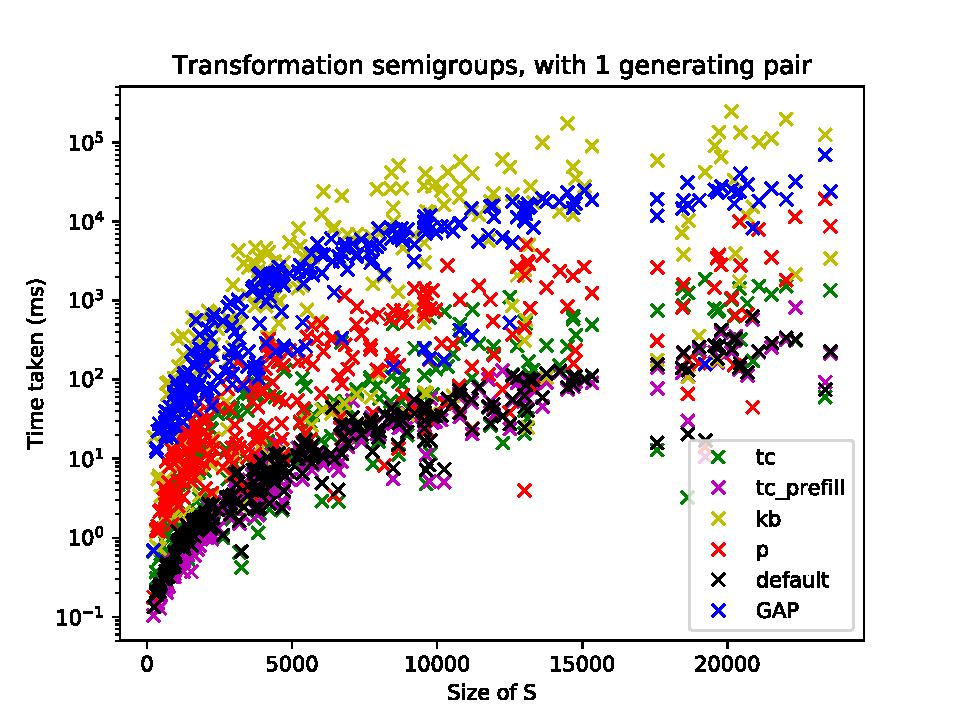
\includegraphics[width=0.9\textwidth]{pics/ch-pairs/bench-trans-1p-times}
  \caption[Benchmark: all algorithms, concrete, 1 pair]
  {Performance of the algorithms on 250 transformation semigroups, with
    one generating pair}
  \label{fig:bench-trans-1p-times}
\end{figure}

\begin{figure}[p]
  \centering
  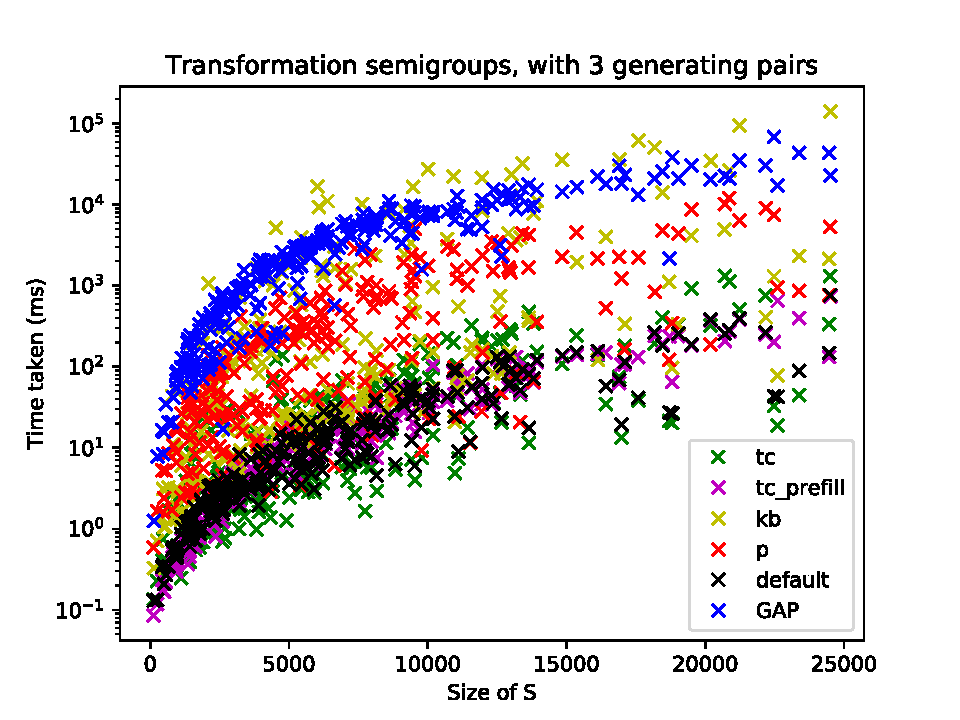
\includegraphics[width=0.9\textwidth]{pics/ch-pairs/bench-trans-3p-times}
  \caption[Benchmark: all algorithms, concrete, 3 pairs]
  {Performance of the algorithms on 250 transformation semigroups, with
    three generating pairs}
  \label{fig:bench-trans-3p-times}
\end{figure}

\begin{figure}[p]
  \centering
  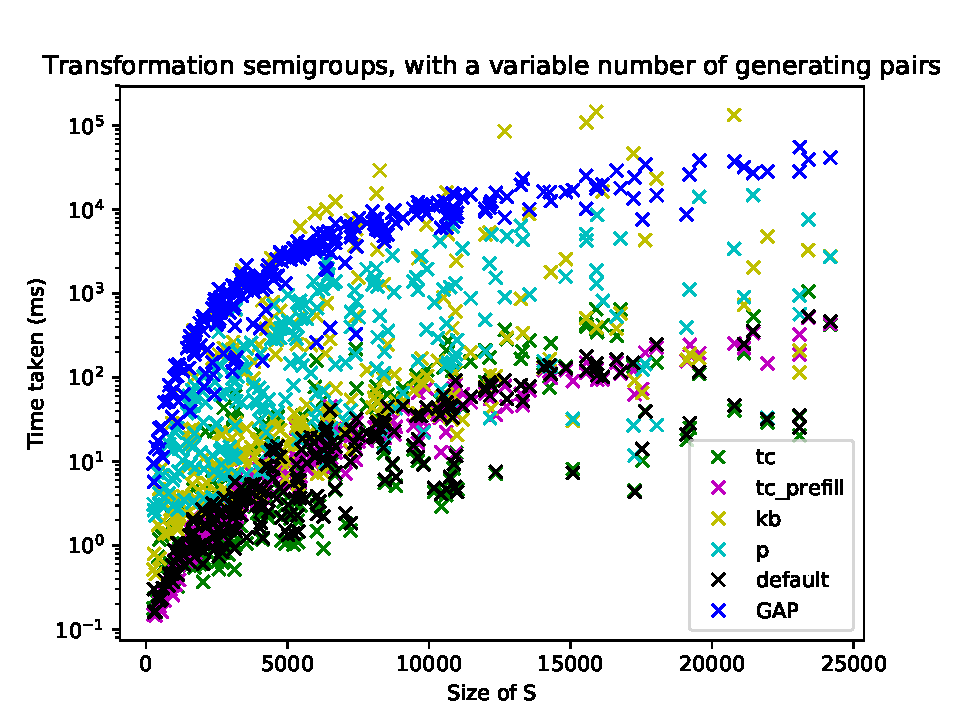
\includegraphics[width=0.9\textwidth]{pics/ch-pairs/bench-trans-vp-times}
  \caption[Benchmark: all algorithms, concrete, $n$ pairs]
  {Performance of the algorithms on 250 transformation semigroups, with
    a variable number of generating pairs}
  \label{fig:bench-trans-vp-times}
\end{figure}

Figure \ref{fig:bench-trans-1p-times} shows the results of a set of $250$ tests
on transformation semigroups.  In each test, $4$ transformations of degree $7$
were chosen at random, and used to generate a semigroup $S$ (any semigroup of
size over $25000$ was rejected).  The elements of $S$ were computed, and a pair
of elements was chosen at random to generate a two-sided congruence $\rho$.  Three more
pairs were chosen at random, and each of the different algorithms described in
this chapter was used to determine whether each pair was contained in $\rho$.

For greater variety, similar tests were also conducted using $3$ generating
pairs for $\rho$, and using a mixture of $1$ to $10$ generating pairs,
as shown in \ref{fig:bench-trans-3p-times} and \ref{fig:bench-trans-vp-times}.
The time taken to return an answer was recorded in each case, and these figures
were compared to one another.  The algorithms used were:
\begin{itemize}
\item the Todd--Coxeter algorithm (\texttt{tc}),
\item the Todd--Coxeter algorithm with pre-filled table (\texttt{tc\_prefill}),
\item the Knuth--Bendix algorithm (\texttt{kb}),
\item pair orbit enumeration (\texttt{p}),
\item the parallel method described in this chapter (\texttt{default}),
\item and the method implemented in the library of \GAP{} (\texttt{GAP}).
\end{itemize}

As can be seen in Figure \ref{fig:bench-trans-1p-times}, the pre-filled
Todd--Coxeter method is the most likely to complete fastest, with the standard
Todd--Coxeter algorithm winning in a sizeable minority of cases.  This backs up the
observations that group theorists have made that the Todd--Coxeter algorithm tends to perform
faster than the Knuth--Bendix algorithm \cite{havascomparing}.  We may also observe that pair
orbit enumeration sometimes completes almost instantly, which makes some sense
when we consider how little work the algorithm does when there are very few
non-reflexive pairs in the congruence.  The Knuth--Bendix procedure lags behind
badly on these examples, taking even longer than the built-in methods in \GAP{}.
These results are a justification for the decision to run only the Todd--Coxeter
algorithms in the case of a concrete representation.

Figures \ref{fig:bench-trans-3p-times} and \ref{fig:bench-trans-vp-times} show
that with a higher number of generating pairs, the pair orbit enumeration
algorithm suffers badly -- this can be understood, since it generally has to
enumerate more pairs when the generating set is larger.  However, with more
generating pairs \texttt{tc} tends to perform relatively better, since there are
likely to be fewer congruence classes and therefore fewer rows in the coset
table.

\begin{figure}[p]
  \centering
  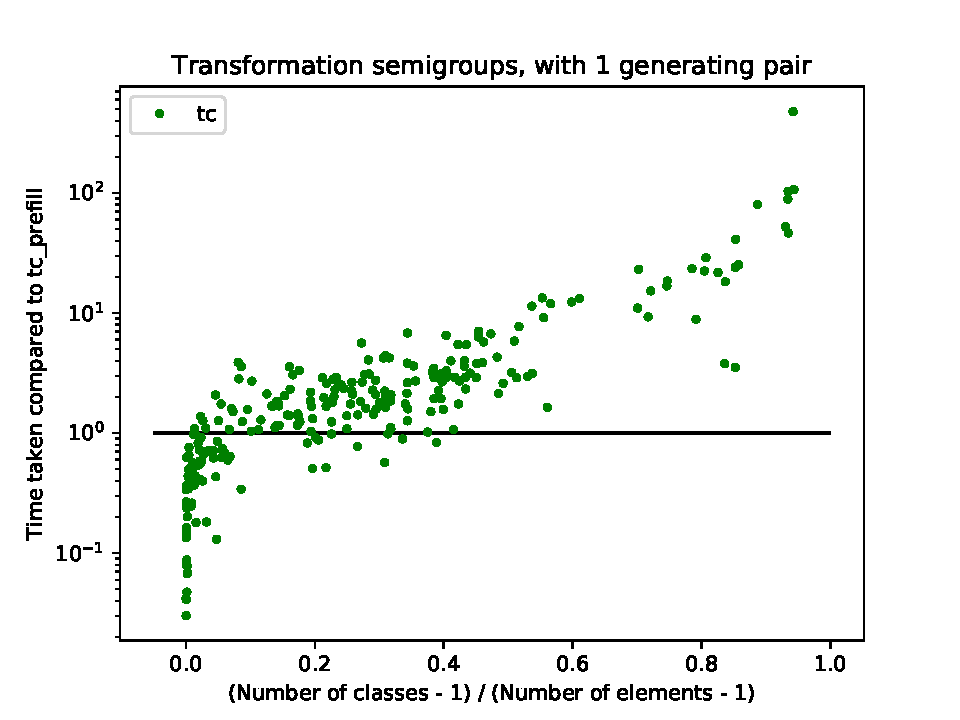
\includegraphics[width=0.9\textwidth]{pics/ch-pairs/bench-trans-tc-1p-tccomp}
  \caption[Benchmark: Todd--Coxeter, concrete, 1 pair]
  {Comparison between the two Todd--Coxeter methods, for transformation
    semigroups with one generating pair}
  \label{fig:bench-trans-tc-1p-tccomp}
\end{figure}

\begin{figure}[p]
  \centering
  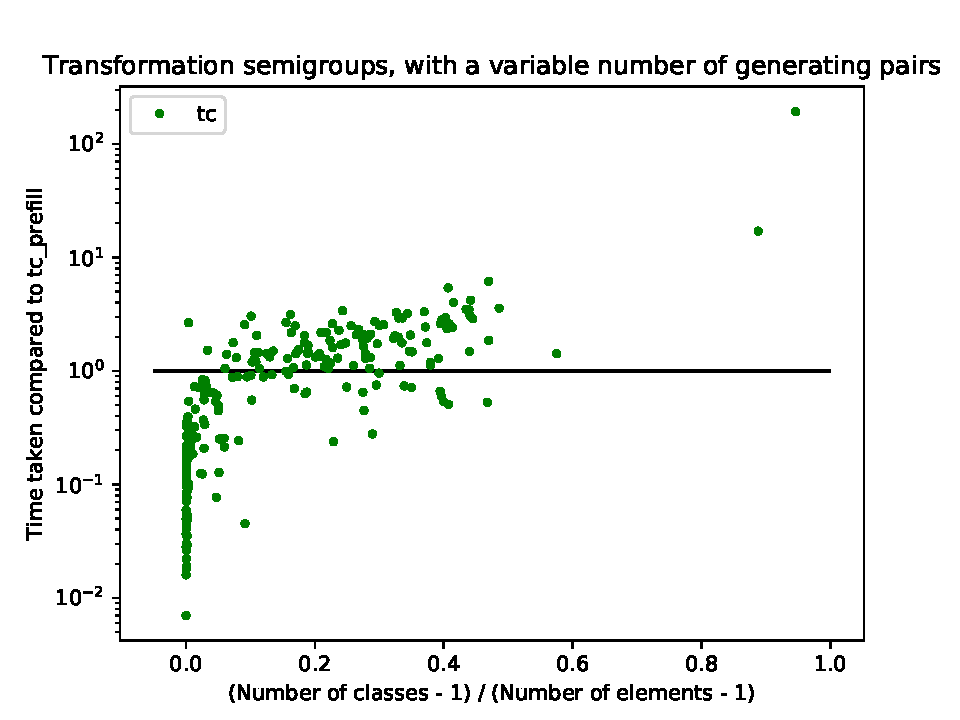
\includegraphics[width=0.9\textwidth]{pics/ch-pairs/bench-trans-tc-vp-tccomp}
  \caption[Benchmark: Todd--Coxeter, concrete, $n$ pairs]
  {Comparison between the two Todd--Coxeter methods, for transformation
    semigroups with a variable number of generating pairs}
  \label{fig:bench-trans-tc-vp-tccomp}
\end{figure}

This tendency is illustrated further in Figures
\ref{fig:bench-trans-tc-1p-tccomp} and
\ref{fig:bench-trans-tc-vp-tccomp}, which show larger tests, each using $5$
generators of degree $8$, and of size up to 100,000.  In these figures we
compare the standard Todd--Coxeter algorithm with the pre-filled version, arranged
according to whether the congruence in question has many or few classes relative
to its size.  The $x$ axis in these figures is
$$(\text{Number of congruence classes} - 1) / (\text{Size of~} S - 1),$$
a scale from $0$ to $1$, where $0$ represents a universal congruence and $1$
represents a trivial congruence.  Since the size of $S$ is a major factor in how
long any algorithm takes to run, only the ratio of \texttt{tc} to
\texttt{tc\_prefill} is shown: a black line is drawn on the graphs to indicate
the length of time taken by \texttt{tc\_prefill}, and a data point is then
plotted for each test, showing how many times as long \texttt{tc} took to
complete.  As can be seen, \texttt{tc} often wins when there are relatively few
large classes, and \texttt{tc\_prefill} is much more likely to win when there are
many small classes.  This reinforces the idea given in Examples \ref{ex:good-tc}
and \ref{ex:good-tc-prefill}, that the winning algorithm may depend on number of
classes, and it is therefore not clear in advance which algorithm may be better.

\begin{figure}[p]
  \centering
  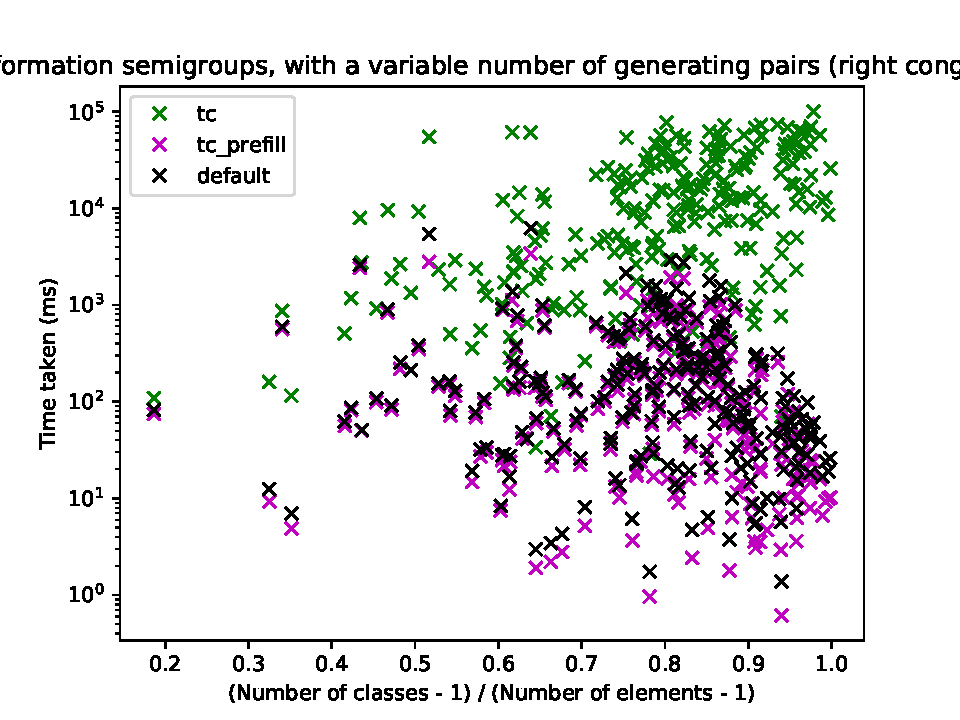
\includegraphics[width=0.9\textwidth]{pics/ch-pairs/bench-trans-tc-vp-right-bynrclasses}
  \caption[Benchmark: Todd--Coxeter, concrete, right, $n$ pairs]
  {Comparison between the two Todd--Coxeter methods, for right
    congruences over transformation semigroups with a variable number of
    generating pairs}
  \label{fig:bench-trans-tc-vp-right-bynrclasses}
\end{figure}

This distinction between the performance of \texttt{tc} and \texttt{tc\_prefill}
is echoed in an example for right congruences, as shown in Figure
\ref{fig:bench-trans-tc-vp-right-bynrclasses}.  Interestingly, it appears that
for right congruences \texttt{tc\_prefill} is even more likely to be effective,
perhaps because in \textsc{ToddCoxeterRight} so little time is spent applying
relations from $W$, so the work is almost finished by the time the table has
been pre-filled.

\begin{figure}[p]
  \centering
  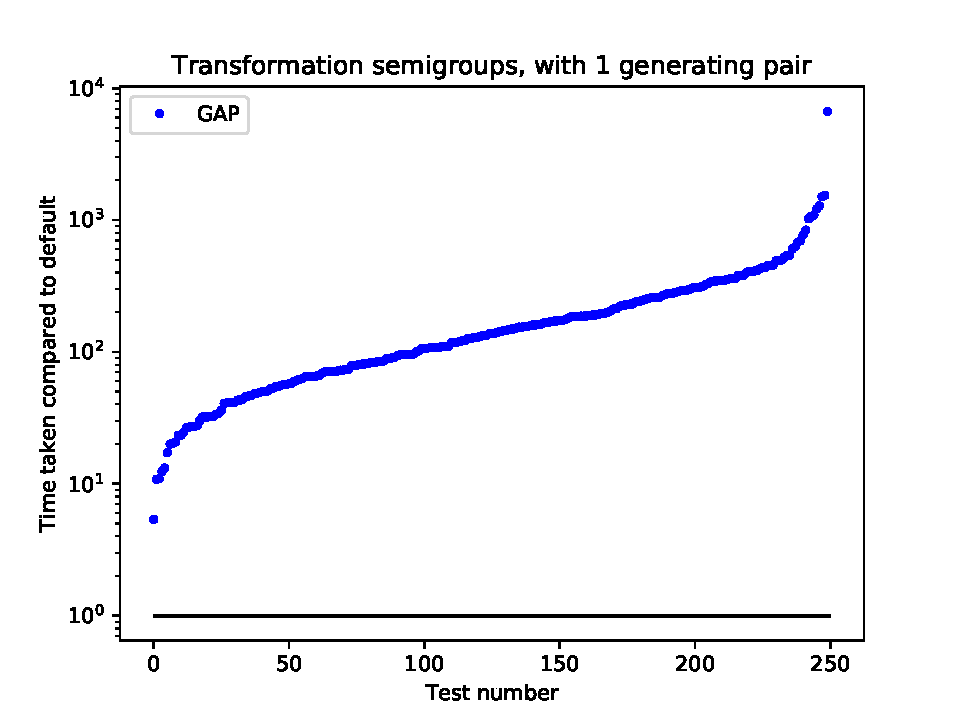
\includegraphics[width=0.9\textwidth]{pics/ch-pairs/bench-trans-1p-gap}
  \caption[Benchmark: \GAP{}/\libsemigroups{}, concrete, 1 pair]
  {Comparison between \libsemigroups{} and the \GAP{} library, for
    transformation semigroups with one generating pair}
  \label{fig:bench-trans-1p-gap}
\end{figure}

\begin{figure}[p]
  \centering
  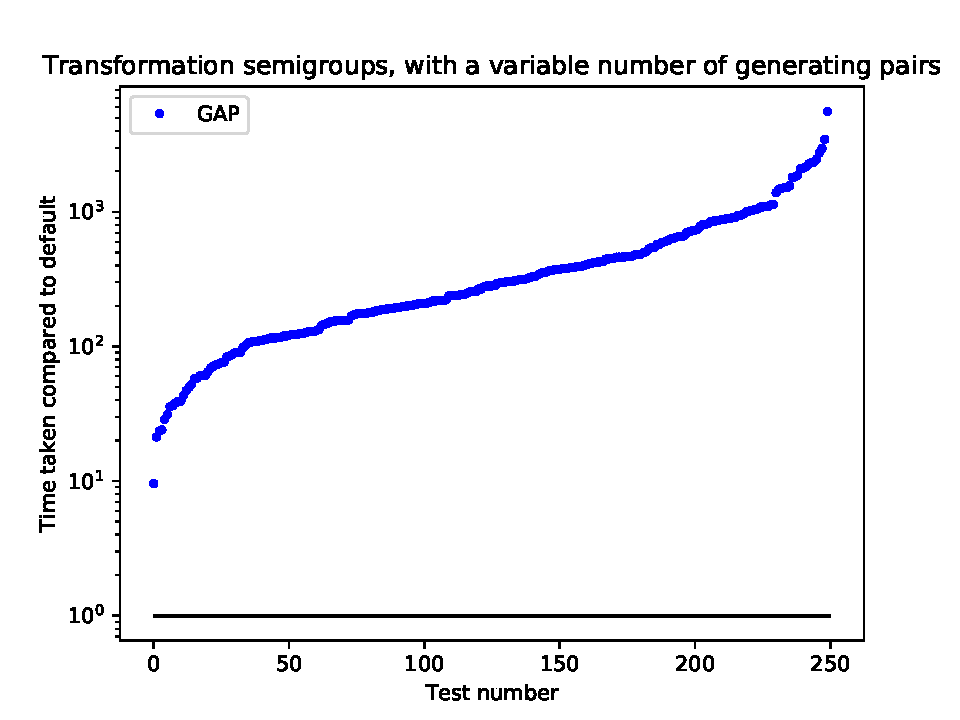
\includegraphics[width=0.9\textwidth]{pics/ch-pairs/bench-trans-vp-gap}
  \caption[Benchmark: \GAP{}/\libsemigroups{}, concrete, $n$ pairs]
  {Comparison between \libsemigroups{} and the \GAP{} library, for
    transformation semigroups with a variable number of generating pairs}
  \label{fig:bench-trans-vp-gap}
\end{figure}

Figures \ref{fig:bench-trans-1p-gap} and \ref{fig:bench-trans-vp-gap} show data
from the same tests, plotted not by
the size of the semigroup, but simply in order of the ratio between \GAP{}'s
runtime and that of the default method in \libsemigroups{}.  As can be
seen, the \libsemigroups{} methods run much faster than the \GAP{} methods in
almost all cases, with the \GAP{} methods taking as much as $7000$ times as long
for one generating pair.  Out of the $500$ tests shown in total in these two
figures, \GAP{} never performed better than \libsemigroups{}.

Further tests were carried out in a similar way, but using finite presentations
instead of concrete representations.  The main difference between these
tests and the ones described previously is that for each transformation
semigroup $S$ that was generated, a finite presentation $\pres X R$ was found
for $S$, and that presentation was used in tests instead of the concrete
representation.  This is intended to test which algorithms are effective
when the elements of the semigroup are not known in advance.
In order to produce a further comparison, the tests for finitely presented
semigroups were also run with the \kbmag{} package for \GAP{} \cite{kbmag}.
The results are shown on the graphs with the name \texttt{kbmag}.

\begin{figure}[p]
  \centering
  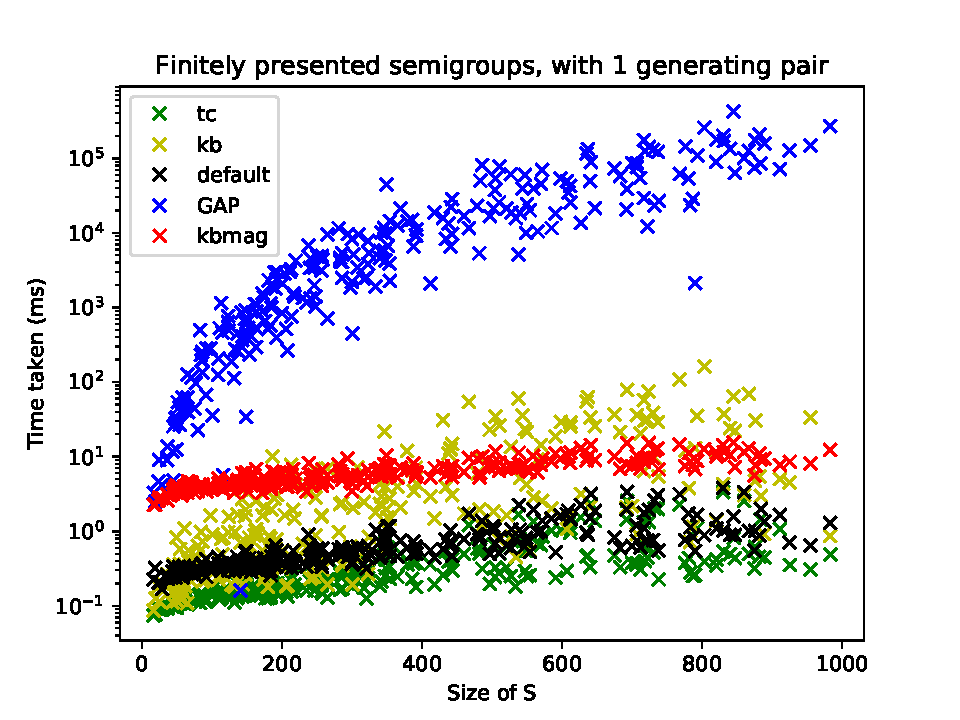
\includegraphics[width=0.9\textwidth]{pics/ch-pairs/bench-fp-1p-times}
  \caption[Benchmark: all algorithms, finitely presented, 1 pair]
  {Performance of the algorithms on $250$ finitely presented semigroups
    with one generating pair}
  \label{fig:bench-fp-1p-times}
\end{figure}

\begin{figure}[p]
  \centering
  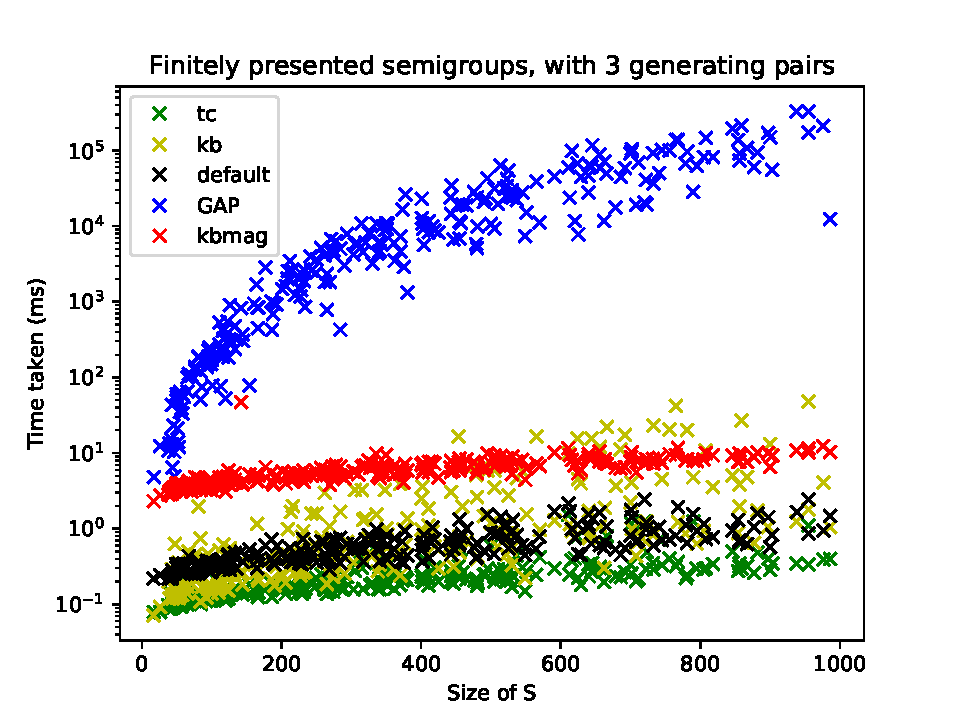
\includegraphics[width=0.9\textwidth]{pics/ch-pairs/bench-fp-3p-times}
  \caption[Benchmark: all algorithms, finitely presented, 3 pairs]
  {Performance of the algorithms on $250$ finitely presented semigroups
    with three generating pairs}
  \label{fig:bench-fp-3p-times}
\end{figure}

\begin{figure}[p]
  \centering
  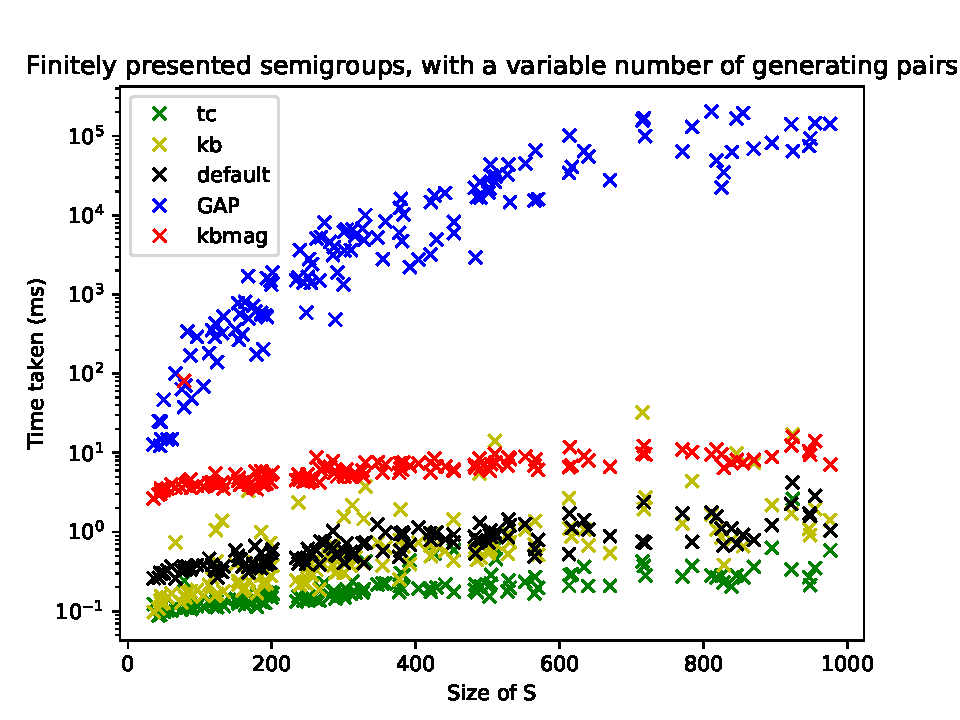
\includegraphics[width=0.9\textwidth]{pics/ch-pairs/bench-fp-vp-times}
  \caption[Benchmark: all algorithms, finitely presented, $n$ pairs]
  {Performance of the algorithms on $250$ finitely presented semigroups
    with a variable number of generating pairs}
  \label{fig:bench-fp-vp-times}
\end{figure}

\begin{figure}[p]
  \centering
  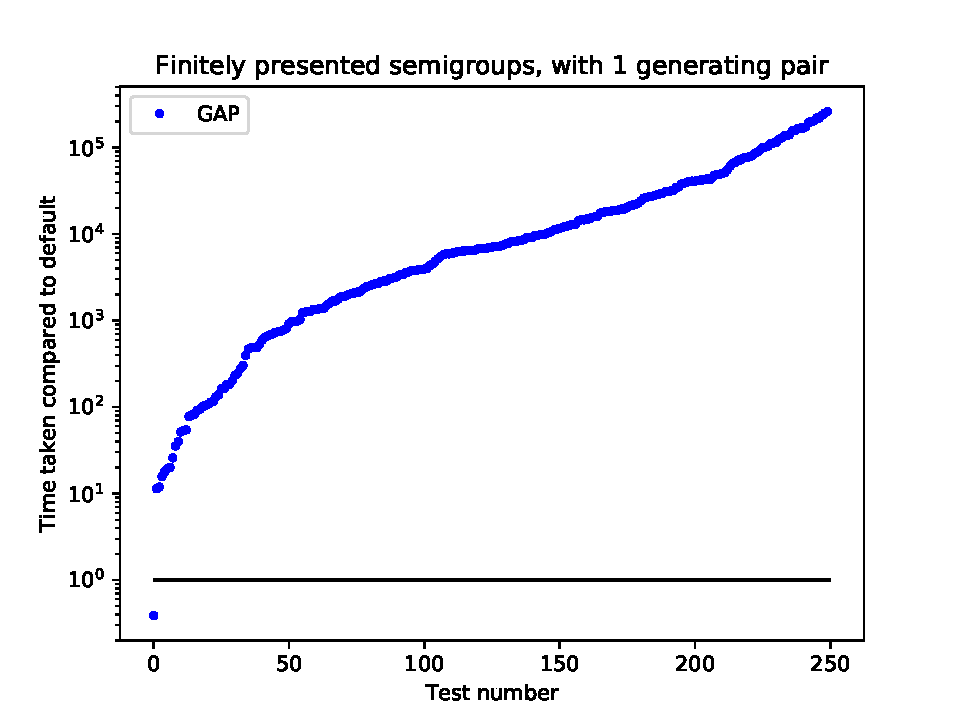
\includegraphics[width=0.9\textwidth]{pics/ch-pairs/bench-fp-1p-gap}
  \caption[Benchmark: \GAP{}/\libsemigroups{}, finitely presented, 1 pair]
  {Comparison between \libsemigroups{} and the \GAP{} library, for
    finitely presented semigroups and one generating pair}
  \label{fig:bench-fp-1p-gap}
\end{figure}

\begin{figure}[p]
  \centering
  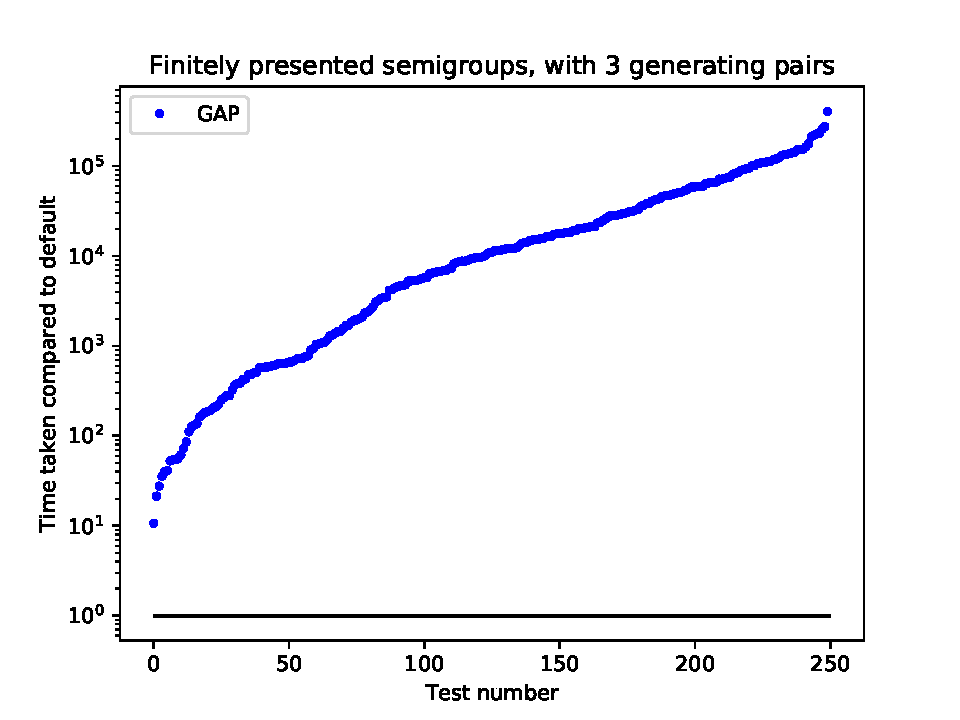
\includegraphics[width=0.9\textwidth]{pics/ch-pairs/bench-fp-3p-gap}
  \caption[Benchmark: \GAP{}/\libsemigroups{}, finitely presented, 3 pairs]
  {Comparison between \libsemigroups{} and the \GAP{} library, for
    finitely presented semigroups and three generating pairs}
  \label{fig:bench-fp-3p-gap}
\end{figure}

\begin{figure}[p]
  \centering
  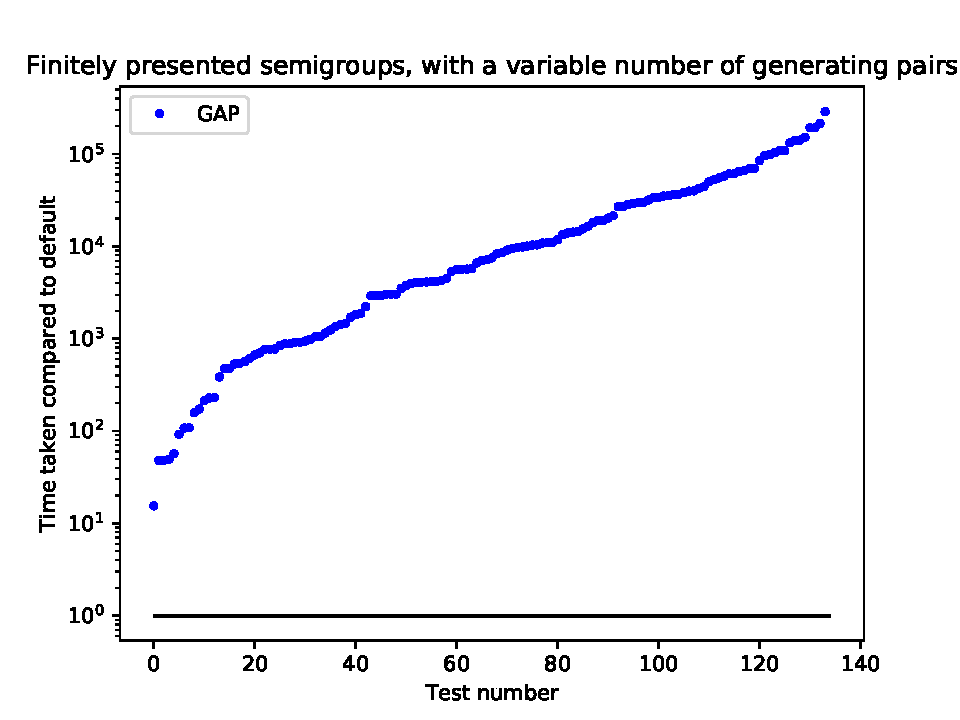
\includegraphics[width=0.9\textwidth]{pics/ch-pairs/bench-fp-vp-gap}
  \caption[Benchmark: \GAP{}/\libsemigroups{}, finitely presented, $n$ pairs]
  {Comparison between \libsemigroups{} and the \GAP{} library, for
    finitely presented semigroups and a variable number of generating pairs}
  \label{fig:bench-fp-vp-gap}
\end{figure}

As can be seen in Figures \ref{fig:bench-fp-1p-gap} to \ref{fig:bench-fp-vp-gap}, the
performance of the \GAP{} library over finite presentations is far worse
than it was for concrete representations, taking as much as 300,000 times as long
as \libsemigroups{} to complete.  Due to the excessive times \GAP{} took to
complete some tests, the size of semigroups was restricted to 1000.  In these
tests, unlike for concrete representations,
the Knuth--Bendix algorithm tended to outperform \GAP{}, but in
general the Todd--Coxeter methods were still faster.  It should be noted, however,
that these were all congruences that were guaranteed in advance to have a finite
number of classes.  An arbitrary congruence on a finitely presented semigroup
may have an infinite number of classes, and there are many examples in which
the Knuth--Bendix algorithm can return an answer but the Todd--Coxeter algorithm cannot (see Example
\ref{ex:good-kbfp}).

\kbmag{} generally performed worse in tests than the Todd--Coxeter algorithm, but was
comparable to our implementation of the Knuth--Bendix algorithm.  It generally took around
$10$ times as long as the complete parallel method (\texttt{default} on the
graphs).

\section{Future work}

The parallel approach described in this chapter is quite open-ended, and could
be extended or improved in several ways.  We will now discuss some areas which
could bear investigation, given more time to spend on the project.

\subsection{Pre-filling the Todd--Coxeter algorithm with a left Cayley graph}
\label{sec:prefill-left}
The pre-filled Todd--Coxeter algorithm, as described in Section
\ref{sec:tc-prefill}, works by starting the procedure with a right Cayley graph
for $S$.  In \libsemigroups{} and in the \Semigroups{} package for \GAP{}, a
right Cayley graph for a semigroup is found using the Froidure--Pin method, which
also returns the corresponding left Cayley graph.  Hence, we may also wish to
find a way to use the left Cayley graph in the pre-filling process.

As mentioned in Section \ref{sec:tc-l-r}, it is possible to use the Todd--Coxeter algorithm
with a reversed multiplication, essentially studying a semigroup anti-isomorphic
to $S$.  It would be possible to apply the same principle, reverse the
multiplication of elements in $S$, and thus use the left Cayley graph instead of
the right Cayley graph in pre-filling.  This could be run as an additional
thread in the parallel procedure.

In many cases, using the left Cayley graph might be very similar in terms of
performance to using the right.  However, some semigroups have left and right
Cayley graphs which are very different.  Consider, for example, the right zero
semigroup $\RZ_n$, which has $n$ generators, $n$ elements, and the
multiplication $xy=y$ for any $x,y \in \RZ_n$.  Its right Cayley graph is the
complete digraph, where any element can be mapped to any other element using the
appropriate generator.  Its left Cayley graph is totally disconnected, with each
vertex $v$ in a single trivial connected component with $n$ edges taking $v$ to
$v$.  With such different left and right Cayley graphs, it seems likely that one
piece of information would be much more helpful than the other in calculating
congruences on the semigroup.

\subsection{Interaction between the Knuth--Bendix and Todd--Coxeter algorithms}
\label{sec:linking-kb-tc}
The Knuth--Bendix and Todd--Coxeter algorithms, as described in this chapter, do
not interact with each other in any way.  The Knuth--Bendix process runs in one
thread, and the Todd--Coxeter process runs in another.  However, information from
one could perhaps be shared with the other.

The main objective of the Knuth--Bendix algorithm is the addition of new rewriting rules to a
rewriting system $\rws$ to satisfy the condition of confluence: if a critical
pair is found, and a new rule $u \to v$ is added to $\rws$, then this gives us a
pair of words $(u,v)$ which represents a pair of congruent elements in the congruence we
are studying.  If a Todd--Coxeter procedure is running in parallel, it would be
possible to send the pair of words $(u,v)$ to the Todd--Coxeter thread, which
at its next convenience would run \textsc{Coinc$\big($Trace($1, u$), Trace($1, v$)$\big)$}
to identify the two corresponding rows in the table.

Conversely, the Todd--Coxeter algorithm may find information which could be used by
the Knuth--Bendix algorithm.  Firstly, it is trivial to record, for each row $i$ of the table,
the word $w_i$ which was first used to describe it: row $1$ is identified with
the empty word ($w_1 := \varepsilon$), and if a row is created using
\textsc{Add($i, x$)} then it is assigned the word $w_ix$.  For each row $i$, we
now have \textsc{Trace}$(1, w_i) = i$; that is, each row has a word which can
act as a representative for its congruence class.
If, in a normal run of the Todd--Coxeter algorithm, it is found that two rows $i$ and $j$
represent the same class and must be combined, then this immediately gives a
pair of words $(w_i,w_j)$ which represent the same congruence class.  This pair
of words can be sent to a parallel instance of the Knuth--Bendix algorithm, which can add it as
a rule $w_i \to w_j$ (or $w_j \to w_i$, as dictated by the chosen ordering).

It may be that this sharing of knowledge between the two algorithms would
greatly increase the speed of certain calculations; or it may be that the time
and space overhead required in the implementation of these ideas would be so great that the
algorithms would not speed up at all.  Experiments with this idea might show it
to be useful, or might suggest that it is not worth pursuing.

\subsection{Using concrete elements in the Todd--Coxeter algorithm}
\label{sec:tc-concrete-elms}
The Todd--Coxeter procedure uses a finite presentation $\pres X R$ and a set of
extra pairs $W$ in order to calculate information about a congruence
over a semigroup $S$.  If $S$ has a concrete representation, then $\pres X R$ and $W$
must be calculated before the beginning of the Todd--Coxeter algorithm, so that the procedure
can use them as parameters.  However, once this information has been calculated,
no other information about $S$ is used for the rest of the algorithm, which only
deals with words, abstract generators and relations.

It may prove helpful to use the concrete representation from $S$ in the the Todd--Coxeter algorithm
procedure, if one is available.  For instance, when \textsc{Add($i, x$)} for some
row $i$ and generator $x$, it would be possible to find an element corresponding
to row $i$, find the element corresponding to the generator $x$, multiply the
two, and see whether a row already exists which represents that element.  In
this way, we can avoid the unnecessary creation of new rows which would only be
deleted by \textsc{Coinc} later.

The pre-filling of Todd--Coxeter tables is one use of the concrete elements that
we have already described and implemented, but they may be many more which would
be effective.

\subsection{Left and right congruences with the Knuth--Bendix algorithm}
\label{sec:kb-l-r}
The parallel method in this chapter, and its implementation in \libsemigroups{},
include support for left congruences and right congruences, as well as the more
important two-sided congruences.  Currently, the Todd--Coxeter and pair enumeration
algorithms are the only methods which support left and right congruences, while
the Knuth--Bendix algorithm is only applied in the two-sided case.  However, there does exist
a version of the Knuth--Bendix algorithm which applies to left and right congruences, and
it could be considered a useful addition to the parallel algorithm described in
this chapter.

The algorithm for right congruences is described in \cite[\S2.8]{sims}, and is
summarised as follows.  Given parameters $X$, $R$, and $W$, as described in
Section \ref{sec:program-inputs}, we wish to find the right congruence $\rho$
defined by $W$ on the semigroup $S$ presented by $\pres X R$.
Our goal is to find a rewriting system $\rws$ which rewrites two words $u$ and
$v$ to the same word if and only if they represent elements of $S$ which are in
the same $\rho$-class.  We define a new symbol, `$\#$', which we will use as an
additional generator in the new alphabet $Y = X \cup \{\#\}$.  We then consider the
pairs in $W$, and produce the set
$$\#W = \{(\#u, \#v) : (u, v) \in W\}.$$
Now, we apply the Knuth--Bendix completion procedure to the presentation
$\pres{Y}{R, \#W}$ in the same way as described in Section \ref{sec:kb}.  The
algorithm produces a rewriting system $\rws$.  Next we consider the subset
$\#X^+ \subseteq Y^+$ defined by
$$\#X^+ = \{\#w : w \in X^+\}.$$
It is shown in \cite[\S2.8]{sims} that $\#X^+$ is a union of
$\lrstar_\rws$-classes, and that the $\lrstar_\rws$-classes contained in $\#X^+$
are in one-to-one correspondence with the $\rho$-classes of $X^+$.  That is,
given a pair of words $(u,v) \in X^+$, the elements $[u]$ and $[v]$ in $S$ lie
in the same $\rho$-class if and only if the words $\#u$ and $\#v$ are rewritten to
the same word by $\rws$.  A symmetric approach would work for left congruences,
with the $\#$ symbols being added to the ends of words instead of to the start.

This additional method could be included in the parallel algorithm, and in
\libsemigroups{}, without too much extra work.  It may be that it would perform
well, returning faster than the Todd--Coxeter algorithm on some examples -- but it would need
to be benchmarked in a manner similar to Section \ref{sec:benchmarking} in order
to establish whether it were worth running in either the concrete case or the
finite presentation case.  Once this were decided, we would be able to remove the
two cross (\xmark) symbols in the `KB' column of Table
\ref{tab:running-in-parallel}, and change each one to either a tick (\cmark) or
a tilde ($\sim$).
